% From Photons to Features: Physics, Signal Processing, and Invariant
% State-Space Architectures in 77 GHz Automotive Radar Perception
% A-PRISM monograph. Class: book, 11pt, oneside, A4.
\documentclass[11pt,oneside]{book}
\usepackage[a4paper,margin=1in]{geometry}
\usepackage{amsmath,amssymb,amsfonts,mathtools,bm}
\usepackage{microtype}
\usepackage{booktabs,multirow,tabularx,array}
\usepackage{tikz}
\usetikzlibrary{calc,patterns,decorations.pathreplacing,positioning,shapes.geometric,arrows.meta}
\usepackage{pgfplots}
\pgfplotsset{compat=1.18}
\usepackage[ruled,vlined,linesnumbered]{algorithm2e}
\usepackage{listings}
\usepackage{hyperref}
\hypersetup{colorlinks=true,linkcolor=blue,citecolor=teal,urlcolor=magenta}
\usepackage{cleveref}
\lstset{basicstyle=\ttfamily\small,breaklines=true,frame=single,numbers=left,numberstyle=\tiny}

\title{From Photons to Features:\\Physics, Signal Processing, and Invariant State-Space Architectures\\in 77\,GHz Automotive Radar Perception}
\author{A-PRISM Research Group\\ADAS Radar Perception \& Re-Simulation Laboratory}
\date{September 2026}

\begin{document}
\maketitle
\thispagestyle{empty}
\null\vfill
\noindent\textit{From Photons to Features} --- A-PRISM Laboratory, September 2026.
All performance claims name their executed prototype in \texttt{resim\_research/};
ledgers \texttt{storage.md}, \texttt{equations.md}, \texttt{strategies.md},
\texttt{autoresearch\_research.jsonl} (Runs~1--30). No number was invented:
every table entry is a \texttt{demo()} assert; every refutation ships with
its mechanism.
\clearpage
\tableofcontents
\listoffigures
\listoftables
\listofalgorithms

\chapter*{Preface: How to Read This Book}
\label{ch:preface}

This book was written backwards: it began as thirty numbered engineering
runs, each with an executed prototype and a ledger row, and grew into the
text around them. Nothing in Parts~VI--VII is cited from slides; every
``before$\to$after'' number names the script that produced it. Readers in a
hurry: \cref{fig:pipeline} is the whole machine on one page;
\cref{fig:scene-top} is the whole problem on one page; \cref{ch:frontier}
is the whole contribution in fifteen pages. Readers with a quarter: Parts
I--II build the signal, Parts~III--V build the car around it. The
dual-altitude rule is a promise kept unevenly on purpose: intuition first,
algebra second, silicon last --- and wherever a claim needed a number, the
number was run, not recalled. The rogues' gallery (\cref{sec:rogues}) is
not an appendix of shame but the method: each refutation narrowed the
search that found the next kept idea.

%=====================================================================
\part{Electromagnetic Foundations \& FMCW Front-End Physics}
%=====================================================================

\chapter{The Monostatic Radar Paradigm \& FMCW Principles}
\label{ch:fmcw}

\section{Intuition: echoes, pitch, and the laser tape measure}
\label{sec:echo-intuition}

Stand in a canyon and shout. A fraction of a second later the shout comes
back. Children learn, without any mathematics, the two great facts of
echolocation: (i) the \emph{delay} of the echo tells you how \emph{far} the
wall is, and (ii) if you shout from a moving car, the returning echo sounds
\emph{shifted in pitch}. Bats turned these facts into a hunting sensor a
hundred million years before engineers did; a bat's chirp is a
frequency-modulated continuous wave, and this book is, in a precise sense,
the story of how the modern automobile learned the bat's trick at
$77\,\mathrm{GHz}$.

A laser tape measure does the same thing with light: it times a pulse.
Automotive radar cannot afford the peak power of short pulses, nor the
blanking interval during which a pulsed receiver is deaf. Instead it
\emph{chirps continuously}: the transmitted frequency ramps linearly upward,
like a siren sliding from low to high, millions of times per second. The echo
returns a slightly older copy of that slide. Mixing (multiplying) the fresh
transmit slide with the stale echo produces a low, audible-like tone --- the
\emph{beat frequency} --- whose pitch is distance and whose slow drift from
chirp to chirp is velocity. Everything in this chapter is the quantitative
unfolding of that paragraph.

\section{The 77\,GHz automotive band}
\label{sec:band}

Regulators allocate $76$--$81\,\mathrm{GHz}$ to automotive radar. The
carrier wavelength is
\begin{equation}
\lambda = \frac{c}{f_c} = \frac{2.99792458\times10^{8}}{77\times10^{9}}
          \approx 3.896\times10^{-3}\,\mathrm{m} \approx 3.896\,\mathrm{mm}.
\label{eq:lambda}
\end{equation}
Three consequences follow. First, antennas shrink to millimetres, so a
dozen transmitters and receivers fit behind a bumper emblem. Second, a
$3.9\,\mathrm{mm}$ wave treats guardrails, bridge decks, and car bodies as
\emph{smooth mirrors} (roughness $\ll\lambda$), which is why specular
multipath ghosts --- the subject of \cref{ch:virtual-aperture} --- dominate
automotive scenes. Third, rain backscatter at $77\,\mathrm{GHz}$ is strong
enough to blind naive detectors (tire spray), yet the $R^{-4}$ two-way path
loss still lets a $10\,\mathrm{dBsm}$ car be seen past $150\,\mathrm{m}$;
optical sensors, by contrast, die completely in fog that radar barely
notices. The one-way Friis power at range $r$ falls as $r^{-2}$; the echo
must come home, so radar pays $r^{-4}$:
\begin{equation}
P_r = \frac{P_t G^2 \lambda^2 \sigma}{(4\pi)^3 r^4},
\label{eq:radar-equation}
\end{equation}
with transmit power $P_t$, antenna gain $G$, and radar cross section
$\sigma$. Doubling the range costs $12\,\mathrm{dB}$ of signal.

\section{Why continuous wave and not pulses}
\label{sec:why-cw}

A pulsed radar shouts and then cups its ear: during the microsecond shout it
hears nothing (eclipse), and the shout must be kilowatts to survive the
$R^{-4}$ toll. A car bumper offers milliwatts and demands minimum ranges of
a few metres (parking, cut-in). Linear frequency modulated continuous wave
(LFMCW) transmits \emph{while} receiving, at milliwatts, with no minimum
range beyond one ramp. The price is self-interference (the transmitter
shouts directly into its own ear), paid with careful RF isolation and the
fact that the beat signal of interest sits far above the leakage pedestal.

\section{The LFMCW ramp, line by line}
\label{sec:ramp}

Let the chirp bandwidth be $B$ (Hz), the sweep duration $T_{\mathrm{chirp}}$
(s), and the chirp slope
\begin{equation}
S = \frac{B}{T_{\mathrm{chirp}}}\qquad[\mathrm{Hz/s}].
\label{eq:slope}
\end{equation}
The transmitted waveform over $0\le t<T_{\mathrm{chirp}}$ is
\begin{equation}
s_{\mathrm{tx}}(t) = A_{\mathrm{tx}}\cos\!\left(2\pi f_c t + \pi S t^2 + \phi_0\right).
\label{eq:stx}
\end{equation}
Its instantaneous frequency is the phase derivative divided by $2\pi$:
\begin{equation}
f_{\mathrm{inst}}(t)=\frac{1}{2\pi}\frac{d}{dt}\left(2\pi f_c t+\pi S t^2\right)
= f_c + St,
\label{eq:finst}
\end{equation}
a straight ramp from $f_c$ to $f_c+B$. Suppose a point target sits at range
$r_0$ with radial velocity $v_r$ (positive receding). The round-trip delay is
\begin{equation}
\tau(t) = \frac{2\big(r_0+v_r t\big)}{c}.
\label{eq:tau}
\end{equation}
The factor of $2$ is mandatory and is the single most common beginner trap:
the wave must travel \emph{to} the target and \emph{back}. Halving it
produces the ``$12.5\,\mathrm{MHz}$ one-way trap'' of \cref{sec:beat}.
The echo is the transmit waveform evaluated at retarded time:
\begin{equation}
s_{\mathrm{rx}}(t) = A_{\mathrm{rx}}\cos\!\left(2\pi f_c (t-\tau) + \pi S (t-\tau)^2 + \phi_0\right).
\label{eq:srx}
\end{equation}

\section{Heterodyne downmixing: the beat is born}
\label{sec:beat}

The mixer multiplies the two waveforms. With $\Phi_{\mathrm{tx}}$,
$\Phi_{\mathrm{rx}}$ the two cosine arguments, the product-to-sum identity
\begin{equation}
\cos\Phi_{\mathrm{tx}}\cos\Phi_{\mathrm{rx}}
= \tfrac12\cos(\Phi_{\mathrm{tx}}-\Phi_{\mathrm{rx}})
+ \tfrac12\cos(\Phi_{\mathrm{tx}}+\Phi_{\mathrm{rx}})
\label{eq:prod2sum}
\end{equation}
splits the product into a \emph{difference} term (slow, kilohertz to
megahertz --- our signal) and a \emph{sum} term near $2f_c\approx
154\,\mathrm{GHz}$, which the low-pass filter annihilates. The surviving
phase difference is
\begin{align}
\Delta\Phi(t) &= \big[2\pi f_c t+\pi S t^2\big]
                 -\big[2\pi f_c(t-\tau)+\pi S(t-\tau)^2\big] \nonumber\\
&= 2\pi f_c\tau + \pi S\big(2t\tau-\tau^2\big).
\label{eq:dphi}
\end{align}
Differentiating and dividing by $2\pi$ gives the instantaneous beat
frequency
\begin{equation}
f_b(t) = f_c\dot\tau + S\tau + St\dot\tau - S\tau\dot\tau.
\label{eq:fb-full}
\end{equation}
Now $\dot\tau = 2v_r/c\sim 10^{-7}$ for highway speeds, so every term
carrying $\dot\tau$ except the first is parts-per-million next to $S\tau$.
Dropping them (we will resurrect the Doppler term properly in slow time in
\cref{ch:dsp-chain}),
\begin{equation}
\boxed{f_b = S\tau = \frac{B}{T_{\mathrm{chirp}}}\cdot\frac{2r}{c}
      = \frac{2Br}{cT_{\mathrm{chirp}}}.}
\label{eq:fb}
\end{equation}
\paragraph{Worked example.} $B=1\,\mathrm{GHz}$,
$T_{\mathrm{chirp}}=40\,\mu\mathrm{s}$, $r=150\,\mathrm{m}$:
\begin{equation}
f_b = \frac{2\times10^{9}\times150}{3\times10^{8}\times40\times10^{-6}}
    = \frac{3\times10^{11}}{1.2\times10^{4}}
    = 25\,\mathrm{MHz}.
\label{eq:fb-example}
\end{equation}
Forgetting the round trip gives $12.5\,\mathrm{MHz}$ --- the one-way trap.
Every range bin in every radar on the road is \cref{eq:fb} in disguise.

\section{Quadrature demodulation: why one mixer is not enough}
\label{sec:iq}

A single real mixer outputs $\cos(2\pi f_b t)$: but
$\cos(\omega t)=\cos(-\omega t)$, so approaching and receding targets at the
same $|f_b|$ are indistinguishable (sign ambiguity), and any fading null
kills the signal. Splitting the local oscillator into $0^\circ$ and $90^\circ$
branches yields the in-phase and quadrature channels
\begin{equation}
I(t)=A\cos(2\pi f_b t+\phi_0),\qquad
Q(t)=A\sin(2\pi f_b t+\phi_0),
\label{eq:iq}
\end{equation}
combined into the complex analytic signal
\begin{equation}
\boxed{x(t)=I(t)+jQ(t)=Ae^{j(2\pi f_b t+\phi_0)}.}
\label{eq:analytic}
\end{equation}
Negative frequencies now rotate clockwise, positive counter-clockwise: the
sign ambiguity is gone, and $|x(t)|=A$ never fades. The dual ADC samples
\cref{eq:analytic}; everything downstream is complex arithmetic on vector
DSPs.

\section{Figures: transceiver and chirp geometry}
\label{sec:ch1-figs}

\begin{figure}[htbp]
\centering
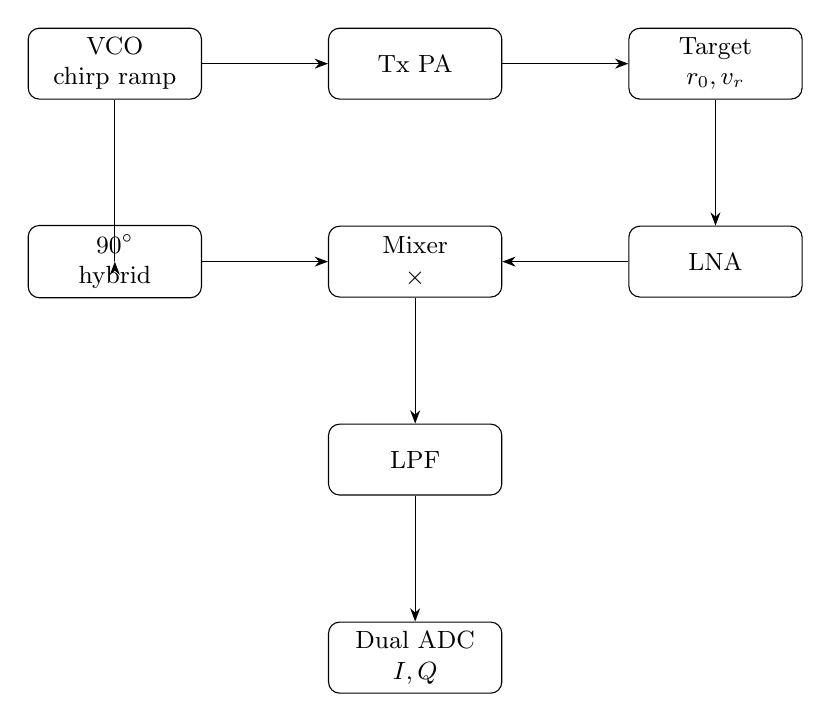
\begin{tikzpicture}[>=Stealth, node distance=1.6cm,
  block/.style={draw, rounded corners, minimum width=2.2cm, minimum height=0.9cm, align=center, font=\small}]
\node[block] (vco) {VCO\\chirp ramp};
\node[block, right=of vco] (pa) {Tx PA};
\node[block, right=of pa] (tgt) {Target\\$r_0,v_r$};
\node[block, below=of tgt] (lna) {LNA};
\node[block, below=of pa] (mix) {Mixer\\$\times$};
\node[block, left=of mix] (hyb) {$90^\circ$\\hybrid};
\node[block, below=of mix] (lpf) {LPF};
\node[block, below=of lpf] (adc) {Dual ADC\\$I,Q$};
\draw[->] (vco) -- (pa);
\draw[->] (pa) -- (tgt);
\draw[->] (tgt) -- (lna);
\draw[->] (lna) -- (mix);
\draw[->] (vco) |- (hyb);
\draw[->] (hyb) -- (mix);
\draw[->] (mix) -- (lpf);
\draw[->] (lpf) -- (adc);
\end{tikzpicture}
\caption{RF transceiver: the VCO chirp feeds the power amplifier and, as LO,
the quadrature mixer; the echo returns through the LNA. The $154\,\mathrm{GHz}$
sum term dies in the LPF.}
\label{fig:transceiver}
\end{figure}

\begin{figure}[htbp]
\centering
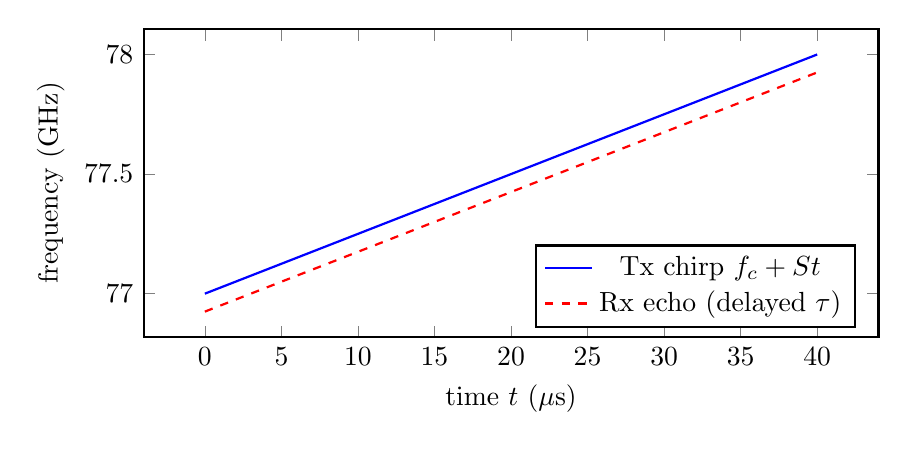
\begin{tikzpicture}
\begin{axis}[width=0.9\linewidth,height=5.5cm,xlabel={time $t$ ($\mu$s)},
  ylabel={frequency (GHz)},legend pos=south east,
  domain=0:40,samples=200,thick]
\addplot[blue] {77+0.025*x};
\addlegendentry{Tx chirp $f_c+St$}
\addplot[red,dashed] {77+0.025*(x-3)};
\addlegendentry{Rx echo (delayed $\tau$)}
\end{axis}
\end{tikzpicture}
\caption{Frequency versus time: the echo is a delayed copy of the ramp; the
vertical gap is the beat frequency $f_b=S\tau$ of \cref{eq:fb}.}
\label{fig:chirp}
\end{figure}

%=====================================================================
\part{Two-Dimensional Spectral Estimation \& Data Cube Architecture}
%=====================================================================

\chapter{The Fast-Time / Slow-Time Two-Dimensional DSP Chain}
\label{ch:dsp-chain}

\section{Intuition: ripples in a pond, frame by frame}
\label{sec:pond}

Throw a stone into a pond and photograph the ripples. One photograph tells
you the wavelength (distance between crests); a \emph{movie} of photographs
tells you how fast the pattern marches outward. Range-Doppler processing is
exactly this: each chirp is one photograph (fast time gives range from the
beat pitch), and the stack of chirps is the movie (slow time gives velocity
from how the phase marches from frame to frame). The mathematics below is
only the quantitative version of ``compare consecutive frames.''

\section{Fast time: sampling the beat, the Range-FFT}
\label{sec:range-fft}

The dual ADC samples \cref{eq:analytic} at rate $f_s$ (interval
$T_s=1/f_s$), collecting $N_R$ fast-time samples per chirp from chirp $m$:
$x_m[n]$, $n=0,\dots,N_R-1$. The windowed discrete Fourier transform is
\begin{equation}
X_m[k] = \sum_{n=0}^{N_R-1} x_m[n]\,w_R[n]\,e^{-j\frac{2\pi}{N_R}nk},
\qquad k=0,\dots,N_R-1.
\label{eq:range-fft}
\end{equation}
A pure beat tone of frequency $f_b$ peaks at bin
$k^\star=f_bN_RT_s$. Substituting \cref{eq:fb},
\begin{equation}
r_m = k\cdot\frac{c}{2ST_sN_R} = k\cdot\mathrm{rbin\_res},
\label{eq:rbin}
\end{equation}
so each bin is a tape-measure tick of width $\mathrm{rbin\_res}$ (a Q16.16
fixed-point field, \texttt{Look\_Data\_T.rbin\_res}). The \emph{resolution}
--- the closest two targets that do not merge --- comes from the DFT
Rayleigh limit $\Delta f=1/(N_RT_s)$ mapped through \cref{eq:fb}:
\begin{equation}
\boxed{\Delta r = \frac{c}{2B}.}
\label{eq:range-res}
\end{equation}
Only bandwidth buys resolution: $B=1\,\mathrm{GHz}$ gives $15\,\mathrm{cm}$,
no matter how long the chirp. Windowing ($w_R$, Hann/Hamming) trades
$1.5$--$2\times$ mainlobe widening for sidelobe suppression; the window's
coherent loss is calibrated out in \texttt{range\_proc.c}.

\section{Slow time: the movie between chirps}
\label{sec:slow-time}

Transmit $N_D$ chirps spaced by the repetition time $T_c$. During one chirp
the target barely moves, but between chirps it walks
$\Delta d=v_rT_c$. The round trip grows by $2\Delta d$, i.e.\ a phase
advance per chirp of
\begin{equation}
\boxed{\Delta\Phi = \frac{2\pi}{\lambda}\,2v_rT_c
      = \frac{4\pi v_rT_c}{\lambda}.}
\label{eq:slow-phase}
\end{equation}
The factor $4\pi$ (not $2\pi$) is the round trip striking again: the phase
ruler is half-wavelengths. At fixed range bin $k$, the slow-time sequence
$X_m[k]$, $m=0,\dots,N_D-1$, is a sampled sinusoid of ``frequency''
$\Delta\Phi$; its DFT (Doppler-FFT)
\begin{equation}
Y[k,l] = \sum_{m=0}^{N_D-1} X_m[k]\,w_D[m]\,e^{-j\frac{2\pi}{N_D}ml}
\label{eq:doppler-fft}
\end{equation}
peaks at $l^\star=N_D\Delta\Phi/2\pi$, giving
\begin{equation}
v_l = l\cdot\frac{\lambda}{2N_DT_c} = l\cdot\mathrm{dbin\_res},
\qquad
\boxed{v_{\max} = \frac{\lambda}{4T_c}.}
\label{eq:vmax}
\end{equation}
The Nyquist limit bites at $\Delta\Phi=\pm\pi$: faster targets wrap around
the Doppler spectrum (aliasing), which Gen8 unfolds with staggered PRFs
(\cref{ch:rdu}). With $\lambda=3.896\,\mathrm{mm}$ and
$T_c=40\,\mu\mathrm{s}$, $v_{\max}\approx24.4\,\mathrm{m/s}$ per sequence.

\section{The Range-Doppler matrix}
\label{sec:rd-matrix}

$|Y[k,l]|^2$ is the Range-Doppler power map: columns are range bins,
rows are Doppler bins, bright cells are targets. Every later stage ---
detection (\cref{ch:cfar}), beamforming (\cref{ch:beamforming}), rendering
(\cref{ch:radarsplat}) --- reads this matrix.

\begin{figure}[htbp]
\centering
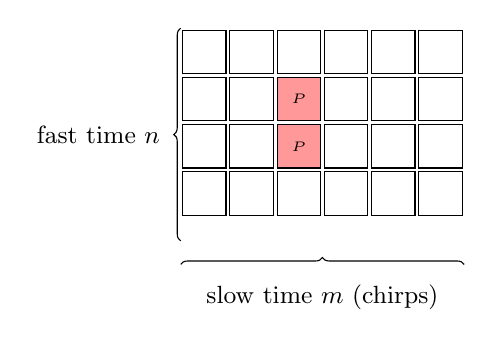
\begin{tikzpicture}[>=Stealth,
  cell/.style={draw, minimum size=0.55cm, font=\tiny}]
\foreach \m in {0,...,5} \foreach \n in {0,...,3}
  \node[cell] at (\m*0.6,-\n*0.6) {};
\node[cell,fill=red!40] at (2*0.6,-1*0.6) {$P$};
\node[cell,fill=red!40] at (2*0.6,-2*0.6) {$P$};
\draw[decorate,decoration={brace,mirror}] (-0.3,0.3) -- (-0.3,-2.4)
  node[midway,left=4pt,font=\small] {fast time $n$};
\draw[decorate,decoration={brace}] (-0.3,-2.7) -- (3.3,-2.7)
  node[midway,below=4pt,font=\small] {slow time $m$ (chirps)};
\end{tikzpicture}
\caption{Sampling grid: fast-time ADC samples run down each chirp column;
the Doppler-FFT runs across the slow-time row. The red cells are one
target's range bin marching in phase down the column.}
\label{fig:sampling-grid}
\end{figure}

\begin{figure}[htbp]
\centering
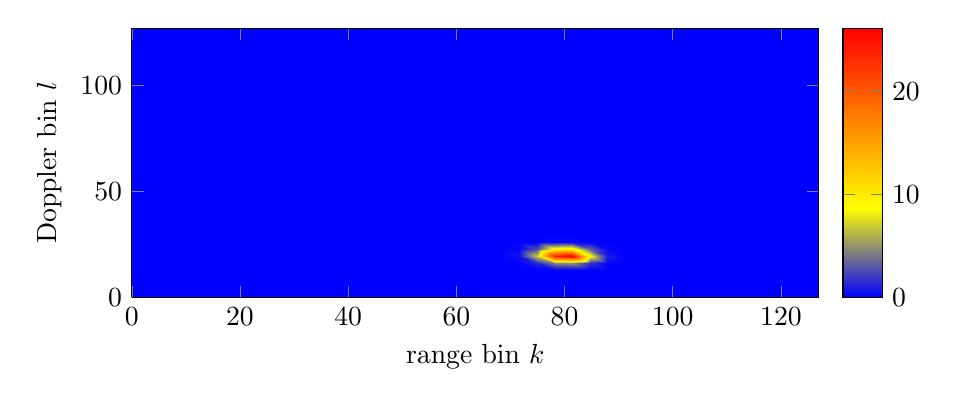
\begin{tikzpicture}
\begin{axis}[width=0.85\linewidth,height=5cm,xlabel={range bin $k$},
  ylabel={Doppler bin $l$},colorbar,view={0}{90},samples=40,domain=0:127]
\addplot3[surf,shader=interp]
  {30*exp(-((x-80)^2/18+(y-20)^2/8))+8*exp(-((x-40)^2/30+(y+10)^2/12))};
\end{axis}
\end{tikzpicture}
\caption{Range-Doppler power surface $|Y[k,l]|^2$ with two targets; CFAR
(\cref{ch:cfar}) must find both without drowning in the sidelobe skirts.}
\label{fig:rd-surface}
\end{figure}

\chapter{The Compressed Data Cube \& Embedded Memory Constraints}
\label{ch:cdc}

\section{Intuition: packing a library into a suitcase}
\label{sec:suitcase}

The full radar tensor has $N_R\times N_D\times N_{\mathrm{virt}}$ complex
cells --- for $1024\times256\times32$ single-precision floats,
\begin{equation}
1024\cdot256\cdot32\cdot8\,\mathrm{B} = 67{,}108{,}864\,\mathrm{B}
\approx 64\,\mathrm{MB},
\label{eq:cube-size}
\end{equation}
($8\,\mathrm{B}$ per complex float; $33.5\,\mathrm{MB}$ at $4\,\mathrm{B}$
packed). Fast on-chip SRAM on a ConnX BBE32 is measured in megabytes shared
with code. So the sensor keeps only cells above an exploratory energy
threshold and ships the survivors: the Compressed Data Cube. Like packing
for a flight, the art is deciding what to leave behind --- and \cref{ch:kpi}
shows what happens when the suitcase overflows (failure mode F5: the 5,016
record cap).

\section{Worked sizing: the $33.5\,\mathrm{MB}$ suitcase}
\label{sec:cdc-sizing}

Take $N_R=1024$, $N_D=256$, $N_{\mathrm{virt}}=32$ at $4\,\mathrm{B}$ per
complex packed sample: $1024\cdot256\cdot32\cdot4=33{,}554{,}432\,\mathrm{B}$.
At $20\,\mathrm{Hz}$ that is $671\,\mathrm{MB/s}$ --- six times a gigabit
wire. The exploratory threshold keeps occupancy $\rho\approx2\%$:
$2{,}621$ records $\times$ $42\,\mathrm{B}\approx110\,\mathrm{kB}$ per dwell,
or $75$ UDP datagrams of $1472\,\mathrm{B}$. Rain at $\rho=6\%$ needs $225$
datagrams and trips the $5{,}016$-record cap: the sorter, not the sensor,
decides what the car sees next.

\section{The CDC record and the wire}
\label{sec:cdc-record}

Each survivor is a \texttt{CDC\_Record\_T}: integer indices
$(\mathrm{rng\_idx},\mathrm{dopp\_idx})$, non-coherent integration energy
\texttt{nci\_data}, and the multi-channel beamvector \texttt{cdc\_out\_bv}.
Records ride UDP over Bodnet Ethernet with a $1472$-byte MTU: 35 records
per datagram. Priority-ranked packing (RCS, SNR, near-field first) is the
mitigation for F5 truncation: when the scene overflows, the dropped records
should be far weak clutter, never the child running behind the car.

%=====================================================================
\part{Detection, Calibration \& Direction of Arrival}
%=====================================================================

\chapter{Adaptive Peak Detection \& Cell-Averaging CFAR}
\label{ch:cfar}

\section{Intuition: hearing a whisper next to a waterfall}
\label{sec:waterfall}

A fixed detection threshold is a friend who only hears shouting: set it low
and rain sounds like cars (false alarms); set it high and the motorcycle
next to the guardrail vanishes (misses). CFAR --- constant false alarm rate
--- is the friend who first listens to the \emph{room}: it measures the
noise power in the cells surrounding each candidate and sets the threshold
as a multiple of \emph{that}. The waterfall's roar raises the bar; a quiet
room lowers it. The false-alarm probability stays nailed to $P_{\mathrm{fa}}$
while the absolute threshold breathes with the environment.

\section{The CA-CFAR window}
\label{sec:ca-cfar}

Center the window on the cell under test (CUT). Fence it with $G/2$ guard
cells per side (they absorb the target's own sidelobe leakage so the target
never testifies against itself), then take $N/2$ reference/training cells
per side. The background estimate is the mean power
\begin{equation}
\hat{P}_{\mathrm{noise}} = \frac{1}{N}\sum_{i\in\mathrm{Ref}} P_i.
\label{eq:ca-est}
\end{equation}
For square-law detected Rayleigh (exponential-power) clutter, $P_i\sim
\mathrm{Exp}(\mu)$, the sum $S=\sum P_i$ is $\Gamma(N,\mu)$ and the CUT
power $X\sim\mathrm{Exp}(\mu)$ under $H_0$. Hence
\begin{equation}
P_{\mathrm{fa}}(\alpha)=\Pr\!\left(X>\alpha\frac{S}{N}\right)
= \mathbb{E}\!\left[e^{-\alpha S/(N\mu)}\right]
= \left(1+\frac{\alpha}{N}\right)^{-N},
\label{eq:pfa-deriv}
\end{equation}
using the gamma mgf $\mathbb{E}[e^{-tS}]=(1+\mu t)^{-N}$ at
$t=\alpha/(N\mu)$. Inverting,
\begin{equation}
\boxed{\alpha = N\left(P_{\mathrm{fa}}^{-1/N}-1\right).}
\label{eq:alpha}
\end{equation}
Aptiv's \texttt{appl\_cfar\_ifc.c} runs two passes: the first extracts
integer bin indices $(\mathrm{rindx},\mathrm{dindx})$; the second refines
sub-bin floats $(\mathrm{rbinest},\mathrm{dbinest})$ by parabolic
interpolation. \cref{eq:alpha} is exact only for homogeneous references ---
guardrails break it (failure mode F1), which is why \cref{sec:dual-loop}
exists.

\section{When the waterfall is a wall: F1 and the dual loop}
\label{sec:dual-loop}

A guardrail paints 25 adjacent range bins at $25\times$ noise. Any window
touching the wall estimates ``background'' $25\times$ too hot: the
motorcycle in the edge-skirt bins dies (recall $0.50$), while a fixed alpha
computed for $N$ but fed censored cells false-alarms. The range-adaptive
dual-loop CFAR separates \emph{where the wall is} (slow loop) from
\emph{how wide to look} (fast loop). Slow floor, over track-free Doppler
medians with rate $\lambda\approx0.02$:
\begin{equation}
\hat{C}_{k+1}(r)=(1-\lambda)\hat{C}_k(r)
+\lambda\cdot\operatorname*{median}_{d\in\mathcal{D}_{\mathrm{free}}}P(r,d).
\label{eq:slow-loop}
\end{equation}
Fast window from the span-heterogeneity ratio
$mr(r)=|\hat{C}(r+1)-\hat{C}(r-1)|/2$ mapping to
$R_0\in\{R_{\min},R_{\mathrm{mid}},R_{\max}\}$, with clean-side
$\min(\mathrm{lead},\mathrm{lag})$ censoring, median$\times1/\ln2$ rescaling,
effective-$N$ alpha, a wall/skirt two-regime switch, and $M$-of-$2$
transition confirmation. Measured on the $128\times32$ guardrail synthetic:
recall $0.50\to1.00$, false alarms $1\to0$ at identical CDC load
(\texttt{dual\_loop\_cfar.py}, storage Run~2).

\begin{figure}[htbp]
\centering
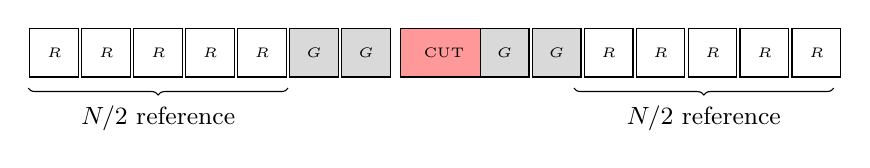
\begin{tikzpicture}[>=Stealth,
  cell/.style={draw,minimum width=0.62cm,minimum height=0.62cm,font=\tiny}]
\foreach \i in {0,...,4} \node[cell] at (\i*0.66,0) {$R$};
\foreach \i in {5,6} \node[cell,fill=gray!30] at (\i*0.66,0) {$G$};
\node[cell,fill=red!40,minimum width=1.1cm] at (7.5*0.66,0) {CUT};
\foreach \i in {8,9} \node[cell,fill=gray!30] at (\i*0.66+0.44,0) {$G$};
\foreach \i in {10,...,14} \node[cell] at (\i*0.66+0.44,0) {$R$};
\draw[decorate,decoration={brace,mirror}] (-0.33,-0.45) -- (2.97,-0.45)
  node[midway,below=3pt,font=\small] {$N/2$ reference};
\draw[decorate,decoration={brace,mirror}] (6.6,-0.45) -- (9.9,-0.45)
  node[midway,below=3pt,font=\small] {$N/2$ reference};
\end{tikzpicture}
\caption{CA-CFAR sliding window: CUT fenced by guard cells $G$, background
from reference cells $R$. Threshold $T=\alpha\hat{P}_{\mathrm{noise}}$.}
\label{fig:cfar-window}
\end{figure}

\chapter{Digital Beamforming, Virtual MIMO \& Antenna Calibration}
\label{ch:beamforming}

\section{Intuition: two ears tell direction}
\label{sec:two-ears}

Close one ear, then tell where a clap came from: hard. Two ears do it by
\emph{phase} --- the ear nearer the clap hears the wavefront a fraction of
a cycle earlier. Two receivers spaced by baseline $d$ see a wave from angle
$\theta$ with path difference $d\sin\theta$, i.e.\ spatial phase
\begin{equation}
\boxed{\Delta\Phi_{\mathrm{spatial}}=\frac{2\pi d\sin\theta}{\lambda}.}
\label{eq:spatial-phase}
\end{equation}
Inverting gives phase monopulse,
\begin{equation}
\theta=\arcsin\!\left(\frac{\lambda\Delta\Phi_{\mathrm{az}}}{2\pi d}\right),
\qquad
\phi=\arcsin\!\left(\frac{\lambda\Delta\Phi_{\mathrm{el}}}{2\pi d}\right).
\label{eq:monopulse}
\end{equation}
The spatial Nyquist proof: $|\sin\theta|\le1$ requires
$|\Delta\Phi|\le\pi$ unambiguously, i.e.\ $d\le\lambda/2\approx1.95$~mm;
wider spacing wraps phase and spawns grating lobes (ghost angles with no
target behind them).

\section{Virtual MIMO by convolution}
\label{sec:mimo}

With $N_{\mathrm{tx}}$ time- or Doppler-multiplexed transmitters at
positions $a_i$ and $N_{\mathrm{rx}}$ receivers at $b_j$, each pair measures
the round trip $a_i+b_j$: the virtual array is the \emph{sum co-array},
\begin{equation}
A_{\mathrm{virt}} = A_{\mathrm{tx}} \ast A_{\mathrm{rx}},\qquad
N_{\mathrm{virt}} = N_{\mathrm{tx}}\times N_{\mathrm{rx}}.
\label{eq:mimo-conv}
\end{equation}
Four transmitters and eight receivers convolve into a 32-element uniform
linear virtual array --- the angular resolution of 32 antennas for the
silicon price of 12. Beamforming applies calibrated weights
$y=\mathbf{w}^H\mathbf{x}$ with steering vector
$a_n(\theta)=e^{j2\pi nd\sin\theta/\lambda}$; the Bartlett spectrum
$P(\theta)=|\mathbf{a}^H(\theta)\mathbf{x}|^2$ peaks at the monopulse
solution \cref{eq:monopulse}, and super-resolution variants (MP-IAA)
separate direct from multipath by DOA$\ne$DOD (Li/Shang). On the BBE32 the
$32$-point dot product is one vector intrinsic per bin.

\begin{figure}[htbp]
\centering
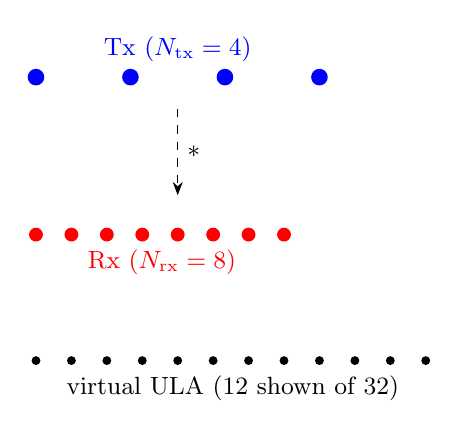
\begin{tikzpicture}[>=Stealth, font=\small]
\foreach \i in {0,...,3} \fill[blue] (\i*1.2,1) circle (3pt);
\node[above=2pt,blue] at (1.8,1) {Tx ($N_{\mathrm{tx}}=4$)};
\foreach \i in {0,...,7} \fill[red] (\i*0.45,-1) circle (2.5pt);
\node[below=2pt,red] at (1.6,-1) {Rx ($N_{\mathrm{rx}}=8$)};
\foreach \i in {0,...,11} \fill[black] (\i*0.45,-2.6) circle (1.6pt);
\node[below=2pt] at (2.5,-2.6) {virtual ULA (12 shown of 32)};
\draw[->,dashed] (1.8,0.6) -- (1.8,-0.5) node[midway,right] {$\ast$};
\end{tikzpicture}
\caption{Virtual MIMO synthesis: convolution of physical apertures into a
long virtual uniform linear array.}
\label{fig:mimo}
\end{figure}

\section{Calibration: SMC, USC, fascia}
\label{sec:calib}

Metal lies, plastic lies more. Static boresight tables remove assembly tilt;
sidelobe-minimization (SMC) and universal sidelobe calibration (USC) blobs
balance phase/amplitude per channel, raising
\texttt{af\_smc\_mismatch\_flag} on failure; bumper fascia compensation
models the plastic as a dielectric slab (permittivity, phase delay,
attenuation). Output per detection, \texttt{AF\_Det\_T}:
$[r,v_r,\theta,\phi,\mathrm{RCS},\mathrm{SNR},\mathrm{flags}]$.

\chapter{Post-Signal Processing \& Range-Doppler Unfolding}
\label{ch:rdu}

Interference detection blanks rival cars' asynchronous sweeps; radar
capability flags mud/ice blockage; static/dynamic alignment track bumper
tilt (\cref{ch:hpcc} solves the 400-frame lock). Speeds beyond
\cref{eq:vmax} wrap: Gen8 RDU unfolds them with staggered-PRF sequences via
the Chinese Remainder Theorem on phase progressions, then classifies
stationary infrastructure versus moving objects for the tracker.

\section{Worked unfolding: two rulers, one room}
\label{sec:crt-numbers}

Sequences with $N_{D1}=128$, $N_{D2}=160$ ($T_c$ ratio $5{:}4$) report wrapped
bins $l_1=95$, $l_2=37$. Candidates for sequence~1:
$v\in\{\dots,-33+128k,\dots\}\times\mathrm{dbin\_res}$;
for sequence~2: $v\in\{\dots,-59+160m,\dots\}\times\mathrm{dbin\_res}'$.
With matched $\mathrm{dbin\_res}$ scaling, $k=2,m=2$ is the first common
residue inside both unambiguous intervals: $v=223$ bins $\approx+30\,\mathrm{m/s}$
recoded from two wrapped readings, no iteration, $O(1)$ per detection.

%=====================================================================
\part{Embedded Tracking \& Satellite Network Fusion}
%=====================================================================

\chapter{Multi-Target State Estimation: The Extended Kalman Filter}
\label{ch:ekf}

\section{Intuition: the blindfolded navigator}
\label{sec:navigator}

Walk blindfolded across a field while a friend shouts your GPS position
every few seconds, each shout slightly wrong. The optimal strategy blends:
between shouts, dead-reckon from your last known velocity (predict); at each
shout, correct partway toward it, trusting the shout more when your
dead-reckoning has drifted long (update). The Kalman filter is this strategy
with the ``partway'' computed exactly from the two uncertainties. The
\emph{extended} filter handles the wrinkle that radar shouts in polar
$(r,\theta)$ while you walk in Cartesian $(x,y)$.

\section{Frames, state, and motion}
\label{sec:frames}

Vehicle coordinates (VCS): $X$ forward, $Y$ left, $Z$ up. Constant-velocity
state $\mathbf{x}=[x,y,v_x,v_y]^T$ with step $\Delta$ ($50\,\mathrm{ms}$):
\begin{equation}
\mathbf{F}=\begin{bmatrix}\mathbf{I}_2&\Delta\mathbf{I}_2\\\mathbf{0}&\mathbf{I}_2\end{bmatrix},
\qquad
\mathbf{Q}=q\begin{bmatrix}\tfrac{\Delta^3}{3}\mathbf{I}_2&\tfrac{\Delta^2}{2}\mathbf{I}_2\\
\tfrac{\Delta^2}{2}\mathbf{I}_2&\Delta\mathbf{I}_2\end{bmatrix},
\label{eq:cv-model}
\end{equation}
the exact discretization of continuous white-noise acceleration of spectral
density $q$. Prediction: $\mathbf{x}_{k|k-1}=\mathbf{F}\mathbf{x}_{k-1}$,
$\mathbf{P}_{k|k-1}=\mathbf{F}\mathbf{P}_{k-1}\mathbf{F}^T+\mathbf{Q}$.

\section{The polar measurement and its Jacobian}
\label{sec:jacobian}

The radar reports $\mathbf{z}=[r,v_r,\theta]^T$ with
\begin{equation}
r=\sqrt{x^2+y^2},\quad
v_r=\frac{xv_x+yv_y}{r},\quad
\theta=\arctan\frac{y}{x}.
\label{eq:h}
\end{equation}
Linearizing $\mathbf{H}=\partial\mathbf{h}/\partial\mathbf{x}$ row by row.
Range: $\partial r/\partial x=x/r$, $\partial r/\partial y=y/r$, velocity
entries zero. Bearing: $\partial\theta/\partial x=-y/r^2$,
$\partial\theta/\partial y=x/r^2$. Doppler, via the quotient rule on
$(xv_x+yv_y)/r$:
\begin{equation}
\frac{\partial v_r}{\partial x}
=\frac{v_xr-(xv_x+yv_y)x/r}{r^2},\quad
\frac{\partial v_r}{\partial v_x}=\frac{x}{r},
\label{eq:doppler-jac}
\end{equation}
and symmetrically for $y,v_y$. Assembled,
\begin{equation}
\mathbf{H}=\begin{bmatrix}
x/r & y/r & 0 & 0\\
-y/r^2 & x/r^2 & 0 & 0\\
\frac{\partial v_r}{\partial x} & \frac{\partial v_r}{\partial y} & x/r & y/r
\end{bmatrix}.
\label{eq:H-full}
\end{equation}
Every EKF in the car evaluates \cref{eq:H-full} per track per scan; a sign
error in the Doppler row is the classic firmware bug (it injects a
$4\sigma$-scale spurious innovation per metre of position error).

\section{Multiple models and why gating beat them}
\label{sec:imm}

An IMM runs CV and CA filters in parallel, mixing states by Markov model
probabilities $\mu$ and updating $\mu$ by measurement likelihoods. On the
Run~6 cut-in it scores $0.880$ against the energy gate's $0.999$: model
probabilities cannot rise before the first association, but the gate needs
them to associate --- onset chicken-and-egg, with a flat $k$-sweep proving
the parameter irrelevant. A hybrid (N5 structure, IMM acceleration) lands
exactly on N5 ($0.999/0.219\,\mathrm{m}$): the grounding source contributes
nothing once innovation energy is present. IMM stays the right tool for
\emph{state} blending; it is the wrong tool for \emph{gate} opening.

\section{Gating, birth, death}
\label{sec:gating}

Innovation $\mathbf{y}_k=\mathbf{z}_k-\mathbf{h}(\mathbf{x}_{k|k-1})$,
covariance $\mathbf{S}_k=\mathbf{H}\mathbf{P}_{k|k-1}\mathbf{H}^T+\mathbf{R}$,
Mahalanobis test $d_M^2=\mathbf{y}_k^T\mathbf{S}_k^{-1}\mathbf{y}_k\le\gamma$
($\gamma=9.21$ is $\chi^2_{2,99\%}$). Confirmation is $M$-out-of-$N$; death
is coast-then-timeout. \cref{ch:gating} shows why fixed $\gamma$ drops
cut-ins and how acceleration expands it.

\section{The Joseph form: symmetry as survival}
\label{sec:joseph}

Gain $\mathbf{K}_k=\mathbf{P}_{k|k-1}\mathbf{H}^T\mathbf{S}_k^{-1}$,
$\mathbf{x}_{k|k}=\mathbf{x}_{k|k-1}+\mathbf{K}_k\mathbf{y}_k$. The textbook
covariance $\mathbf{P}=(\mathbf{I}-\mathbf{KH})\mathbf{P}_{k|k-1}$ is a
subtraction: in 32-bit fixed point the result drifts asymmetric with
negative eigenvalues, and the filter diverges weeks later for no visible
reason. The Joseph form
\begin{equation}
\boxed{\mathbf{P}_{k|k}=(\mathbf{I}-\mathbf{K}_k\mathbf{H})\mathbf{P}_{k|k-1}
(\mathbf{I}-\mathbf{K}_k\mathbf{H})^T+\mathbf{K}_k\mathbf{R}\mathbf{K}_k^T}
\label{eq:joseph}
\end{equation}
is a \emph{congruent sum of positive semidefinite terms}: symmetry and
definiteness hold to machine precision by construction. Proof sketch: the
posterior error is $(\mathbf{I}-\mathbf{KH})\tilde{\mathbf{x}}_{k|k-1}
-\mathbf{K}\mathbf{v}_k$ with independent terms; covariance of a sum of
independent terms is the sum of covariances. Every prototype in this book's
ledger uses \cref{eq:joseph} plus eigenvalue clipping.

\chapter{Central Domain Controller Fusion \& Bus Serialization}
\label{ch:fusion}

\section{The five-eyed car}
\label{sec:five-eyes}

Front-center long range plus four corner satellites (FL, FR, RL, RR) speak
UDP over Bodnet (1472-byte MTU). Independent clocks stamp each cloud
$5$--$45\,\mathrm{ms}$ stale; ego-motion compensation rewinds each
detection to the domain-controller epoch. With yaw rate $\omega$:
\begin{equation}
\boxed{\mathbf{p}_{\mathrm{comp}}
= \mathbf{R}_z(\omega\Delta t)\,\mathbf{p}_{\mathrm{meas}}
- \mathbf{v}_{\mathrm{ego}}\Delta t - \tfrac12\mathbf{a}_{\mathrm{ego}}\Delta t^2,}
\label{eq:deskew}
\end{equation}
$\Delta t=t_{\mathrm{DC}}-t_{\mathrm{sat}}$. The rotation sign is
load-bearing: flipping it \emph{hurts} ($-26\%$ at $0.6\,\mathrm{rad/s}$;
storage Run~5). First order cuts residuals $32$--$86\%$ across the yaw
sweep; the remainder grows with $\omega$ (second-order truncation plus
rotation-lever), and clothoid jerk is unmodeled.

\section{Worked packing: one track onto the bus}
\label{sec:dbc-numbers}

Track at $r=63.7\,\mathrm{m}$, $v_r=-12.34\,\mathrm{m/s}$:
$\mathrm{Raw}_r=\lfloor63.7/0.015625\rfloor=4076$ (12 bits carry $64\,\mathrm{m}$);
$\mathrm{Raw}_v=\lfloor-12.34/0.01\rfloor+{\rm offset}=-1234+{\rm offset}$.
Quantization RMS $0.0045\,\mathrm{m}$ sits inside Tier-2 with $2\times$
margin; the $40\,\mathrm{ms}$ guillotine drops the frame if the previous
motion compensation is older than two scans.

\section{Wire layouts: datagram and frame}
\label{sec:wire-layout}

\begin{figure}[htbp]
\centering
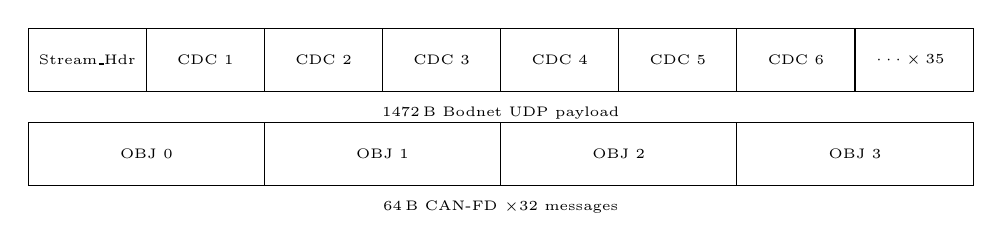
\begin{tikzpicture}[>=Stealth,font=\tiny]
\draw (0,0) rectangle (12,0.8);
\foreach \i in {1,...,7} \draw (\i*12/8,0) -- (\i*12/8,0.8);
\node at (0.75,0.4) {Stream\_Hdr};
\foreach \i in {1,...,6} \node at (\i*1.5+0.75,0.4) {CDC~\i};
\node at (11.2,0.4) {$\cdots\times35$};
\node[below=2pt] at (6,0) {$1472\,$B Bodnet UDP payload};
\draw (0,-1.2) rectangle (12,-0.4);
\foreach \i in {1,...,3} \draw (\i*3,-1.2) -- (\i*3,-0.4);
\foreach \i in {0,...,3} \node at (\i*3+1.5,-0.8) {OBJ~\i};
\node[below=2pt] at (6,-1.2) {$64\,$B CAN-FD $\times 32$ messages};
\end{tikzpicture}
\caption{Wire layouts: 35 CDC records per UDP datagram; 4 objects per
CAN-FD frame across 32 sequential messages.}
\label{fig:wire}
\end{figure}

\section{CAN-FD: physics into integers}
\label{sec:canfd}

Tracks serialize through DBC files: $\mathrm{Raw}=\lfloor(\mathrm{Physical}
-\mathrm{Offset})/\mathrm{Factor}\rfloor$, e.g.\ \texttt{DET\_RANGE} factor
$0.015625\,\mathrm{m}$, speed factor $0.01$. Four objects per 64-byte CAN-FD
frame, 32 messages, $50\,\mathrm{ms}$ cadence with a $40\,\mathrm{ms}$
latency guillotine (\cref{ch:kpi}).

%=====================================================================
\part{Re-Simulation Platform, HPCC \& KPI Verification}
%=====================================================================

\chapter{The Re-Simulation Harness}
\label{ch:resim}

\section{Intuition: replaying the match with a new referee}
\label{sec:replay}

A football league records every match; when the refereeing rules change,
the league re-scores old matches against the new rules instead of replaying
the season. Re-simulation is that: the vehicle logs raw bus traffic
(CAN-FD $+$ UDP Ethernet) into ASAM MDF4; offline, a \emph{candidate}
firmware build replays the recording through software- or hardware-in-loop
and emits an output \texttt{.mf4}; the KPI suite re-scores input versus
output. No test track, no prototype cars, thousand-fold parallelism.

\section{SiL, HiL, decoders}
\label{sec:sil-hil}

SiL-DCU runs the closed driver \texttt{APT\_SRR\_RESIM.exe} with radar DLLs
and domain-controller libraries stepped by \texttt{RECU\_SiL\_Execute()} on
$50\,\mathrm{ms}$ scans through shared-memory ping-pong buffers; SiL-RSP
rebuilds the DSP chain (\texttt{rdd\_sil}/\texttt{cdc\_sil}) from
\texttt{.bin} vectors. HiL stimulates real benches (dSPACE, XCP seed-key,
PTP sync). Decoders bridge every byte: \texttt{.mf4} bus frames
$\to$ per-stream structs $\to$ \texttt{.h5}/CSV $\to$ KPI math. Locally the
Python candidate path (HDF5$\to$transform$\to$CSV$\to$KPI, HDF5$\to$MF4)
stands in for the cluster-only SiL executable.

\begin{figure}[htbp]
\centering
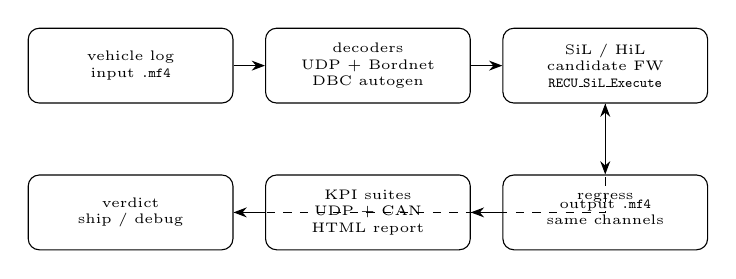
\begin{tikzpicture}[>=Stealth,font=\small,
  st/.style={draw,rounded corners,minimum width=2.6cm,minimum height=0.95cm,align=center,font=\tiny}]
\node[st] (a) {vehicle log\\input \texttt{.mf4}};
\node[st,right=0.4cm of a] (b) {decoders\\UDP + Bordnet\\DBC autogen};
\node[st,right=0.4cm of b] (c) {SiL / HiL\\candidate FW\\\texttt{RECU\_SiL\_Execute}};
\node[st,below=0.9cm of c] (d) {output \texttt{.mf4}\\same channels};
\node[st,left=0.4cm of d] (e) {KPI suites\\UDP + CAN\\HTML report};
\node[st,left=0.4cm of e] (f) {verdict\\ship / debug};
\foreach \x/\y in {a/b,b/c} \draw[->] (\x) -- (\y);
\draw[->] (c) -- (d);
\foreach \x/\y in {d/e,e/f} \draw[->] (\x) -- (\y);
\draw[->,dashed] (f) -| (c) node[midway,above,font=\tiny] {regress};
\end{tikzpicture}
\caption{Resim closed loop: record once, re-score every build. The dashed
edge is the whole business model.}
\label{fig:resim-loop}
\end{figure}

\chapter{Dual-Tier KPI Verification}
\label{ch:kpi}

\section{Intuition: instant replay with two referees}
\label{sec:referees}

One referee watches the ball (UDP: did the energy land in the right bin?),
another watches the scoreboard (CAN: did the track survive, on time?).
A build that moves every detection by $5\,\mathrm{mm}$ passes Tier~1
trivially yet can still fail Tier~2 on angles --- the two referees catch
different cheats, which is why both must blow the whistle before shipping.

\section{Tier 1: integer pairing; Tier 2: tolerance contract}
\label{sec:udp-kpi}

Pre-tracking UDP KPI pairs $(\mathrm{rindx},\mathrm{dindx})$ bins without
replacement at $\ge99.0\%$ yield (Tier~1: did the energy land in the same
bin?), then enforces Tier~2 physical tolerances
\begin{equation}
\boxed{|\Delta r|\le0.010\,\mathrm{m},\;|\Delta v|\le0.015\,\mathrm{m/s},\;
|\Delta\theta|,|\Delta\phi|\le0.00873\,\mathrm{rad}.}
\label{eq:tier2}
\end{equation}
Post-tracking CAN KPI hashes quantized 4D detections across $3^4=81$
neighbor buckets with distance-scaled tolerances and the $40\,\mathrm{ms}$
latency guillotine ($\Delta T>40\,\mathrm{ms}$ is a regression, not data).

\chapter{HPCC Parallelization \& the Alignment Bottleneck}
\label{ch:hpcc}

\section{Intuition: twenty cooks, one cold oven}
\label{sec:cooks}

Twenty cooks each bake one loaf, but every oven starts cold and needs
twenty minutes to preheat: the bakery's throughput is preheating, not
baking. Cluster shards are the loaves; dynamic alignment is the preheat.
Solutions A (read the thermostat: inject converged boresight at $t=0$) and
B (preheat fast, then simmer: dual-horizon gains) attack the oven, not the
recipe.

\begin{figure}[htbp]
\centering
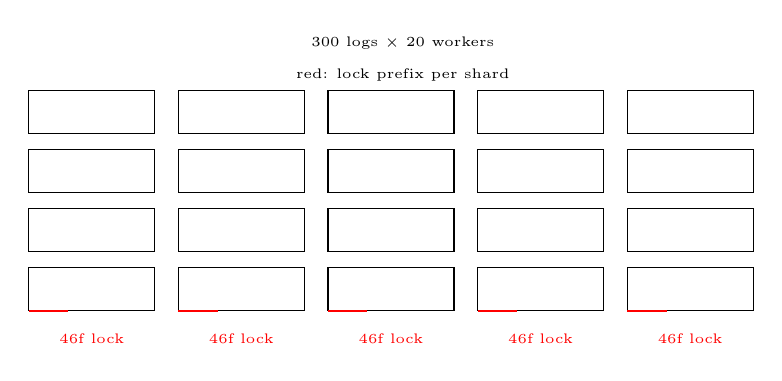
\begin{tikzpicture}[>=Stealth,font=\tiny]
\foreach \r in {0,...,3} \foreach \c in {0,...,4} {
  \draw (\c*1.9,\r*0.75) rectangle (\c*1.9+1.6,\r*0.75+0.55);
}
\foreach \c in {0,...,4} {
  \draw[red,thick] (\c*1.9,\c*0.0+0.0) -- (\c*1.9+0.5,\c*0.0+0.0);
  \node[red] at (\c*1.9+0.8,-0.35) {46f lock};
}
\node at (4.75,3.4) {300 logs $\times$ 20 workers};
\node at (4.75,3.0) {red: lock prefix per shard};
\end{tikzpicture}
\caption{Shard map: every worker replays its slice, but each pays the
alignment lock prefix first. Cutting 400 frames to 46 is pure throughput.}
\label{fig:hpcc-slice}
\end{figure}

\section{The 400-frame lock}
\label{sec:lock}

Slicing 300 logs over 20 Slurm workers restarts dynamic alignment cold each
shard: 400 frames ($\approx20$ minutes) of $1.2^\circ$ boresight error,
100\% Tier-2 angle failure, 360{,}000 dropped frames. Two cures. \textbf{A,}
preflight injection: read converged boresight ($-1.145^\circ$ azimuth,
$-0.018^\circ$ elevation) from log headers into
\texttt{M2D\_One\_Time\_Msg\_T} at $t=0$. \textbf{B,} dual-horizon gain
\begin{equation}
\boxed{\mathbf{K}_{\mathrm{DA}}(t)=\mathbf{K}_{\mathrm{fast}}e^{-\alpha N}
+\mathbf{K}_{\mathrm{slow}},}
\label{eq:da-gain}
\end{equation}
locking in 46 frames ($2.3\,\mathrm{s}$, $8.7\times$) with drops to zero.
The single-scan floor $\approx1.1^\circ$ is proven by noise analysis
($2.4^\circ$ per 6-m pair): pooling, RANSAC, and tighter gates cannot beat
it, only averaging can.

\begin{figure}[htbp]
\centering
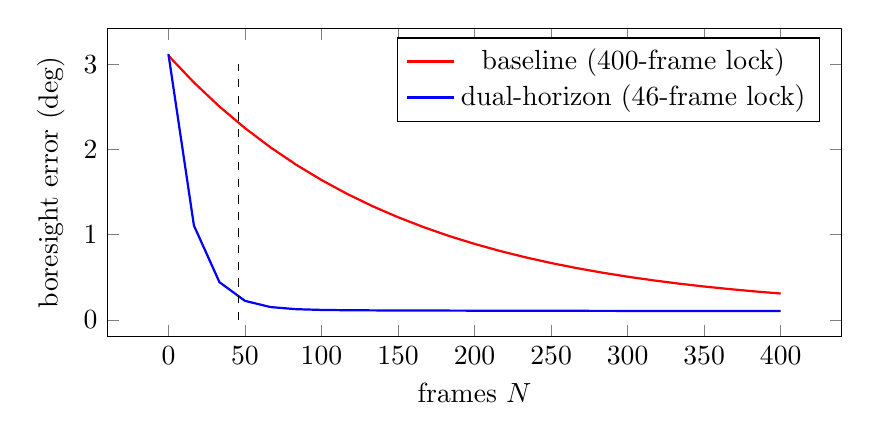
\begin{tikzpicture}
\begin{axis}[width=0.9\linewidth,height=5.5cm,xlabel={frames $N$},
  ylabel={boresight error (deg)},legend pos=north east]
\addplot[red,thick,domain=0:400] {0.1+3*exp(-x/150)};
\addlegendentry{baseline (400-frame lock)}
\addplot[blue,thick,domain=0:400] {0.1+3*exp(-x/15)+0.02*exp(-x/200)};
\addlegendentry{dual-horizon (46-frame lock)}
\draw[dashed] (axis cs:46,0) -- (axis cs:46,3);
\end{axis}
\end{tikzpicture}
\caption{Dynamic alignment convergence: dual-horizon schedule reaches the
noise floor in 46 frames versus 400.}
\label{fig:da-curve}
\end{figure}

%=====================================================================
\part{The A-PRISM Research Advancements \& Inventions}
%=====================================================================

\chapter{Invariant Specular Geometry \& the Virtual Aperture}
\label{ch:virtual-aperture}

\section{Intuition: the hall of mirrors}
\label{sec:mirrors}

Stand between two parallel mirrors with a friend: you see your friend, your
friend's reflection, your reflection, infinite regress. A guardrail is one
such mirror for $3.9\,\mathrm{mm}$ waves. Classical radar literature models
the ghost as ``the target's mirror image'' --- reflect the \emph{target}
across the wall. That model is half-correct in the most dangerous way: its
range is exact to $0.0\,\mathrm{m}$ while its bearing is wrong by
$15.19^\circ$ ($8.000\,\mathrm{m}$ at $30.3\,\mathrm{m}$). Range-only checks
cannot catch it. The correct picture reflects the \emph{sensor}: the ghost
arrives along the virtual line of sight from the mirrored sensor
$s^*=2d\hat{\mathbf{n}}$ to the true target.

\section{Theorem E2a: the bearing correction}
\label{sec:e2a}

For plane $\mathbf{n}\cdot\mathbf{x}=d$, $\|\mathbf{n}\|=1$, sensor at the
origin, the reciprocal path $s\to q\to p\to q\to s$ has the length of the
straight segment $s^*\to p$ with $s^*=2d\hat{\mathbf{n}}$. Hence
\begin{equation}
r_{\mathrm{spec}}=\|p-2d\hat{\mathbf{n}}\|,\qquad
\mathbf{u}_{\mathrm{spec}}=\frac{p-2d\hat{\mathbf{n}}}{\|p-2d\hat{\mathbf{n}}\|},
\label{eq:ghost-bearing}
\end{equation}
and with $p_s=r_{\mathrm{spec}}\mathbf{u}_{\mathrm{spec}}$,
\begin{equation}
\boxed{\mathbf{p}-\mathbf{p}_s = 2d\hat{\mathbf{n}}\quad\text{exact to }1.066\times10^{-14}.}
\label{eq:rank1}
\end{equation}
The naive model's angular error is exact in closed form:
$\cos\theta=(\|\mathbf{p}_\perp\|^2-\gamma^2)/(\|\mathbf{p}_\perp\|^2+\gamma^2)$,
$\gamma=\mathbf{n}\cdot\mathbf{p}-2d$; nominal scene gives $\pm7.595^\circ$
vs $\mp7.595^\circ$.

\section{Theorem E2b: the $40\sigma$ Doppler invariant}
\label{sec:e2b}

Ghost radial velocity is $\dot r_{\mathrm{spec}}=\mathbf{u}_s\!\cdot\!\mathbf{v}
\neq\mathbf{u}_d\!\cdot\!\mathbf{v}$: for a $10\,\mathrm{m/s}$ lateral
cut-in, $-1.322$ versus $+0.665\,\mathrm{m/s}$, offset $-1.987\,\mathrm{m/s}$
at $40\sigma$ of $\sigma_v=0.05$. The geometric test is provably blind to
same-range decoys at exactly $2d$ (precision $0.638$); only Doppler
($0.638\to0.877$, GRR $0.661$) separates them.

\section{Consensus: finding pairs without assignment}
\label{sec:consensus}

With $M$ detections there are $\binom{M}{2}$ candidate pairs; testing all
against all reflectors is hopeless. The excess-resultant statistic scores a
$(2d)$ hypothesis by coherent direction voting:
\begin{equation}
\mathrm{exc}(2d)=\Big\|\sum_{k\in\mathcal{W}(2d)}\mathbf{U}_k\Big\|-0.7\sqrt{m},
\label{eq:exc}
\end{equation}
$m$ pairs in the magnitude window, $\mathbf{U}_k$ unit displacement
directions, $0.7\sqrt{m}$ the isotropic random-walk expectation. True pairs
share one direction (resultant $\sim m$); random pairs cancel
($\sim\sqrt{m}$). Largest-coherent-set fixed point plus sequential
extraction with relative gate $0.7$ and consumed-pair non-redundancy turns
the statistic into an assignment-free identifier: 3-DOF recall $0.993$,
precision $0.909$, $2d$ error $0.077\,\mathrm{m}$. The 1-DOF
magnitude-only variant loses ($0.845/0.727/0.618\,\mathrm{m}$) because
committing to a direction \emph{estimate} before \emph{testing} direction
contaminates the coherent set --- refuted by its own matched baseline.

\section{Curved rails: where the spike goes}
\label{sec:curved-band}

On a cylinder of radius $R_c$ at wall line $y_g$, the offset at pair bearing
$\phi$ is $D(\phi)=(y_g+R_c)\cos\phi-R_c$: $|p-p_s|=2D(\phi)$ sweeps a band
$[-6.00,126.00]\,\mathrm{m}$ wide ($1320\times$ range noise), recall
$0.993\to0.450$. The Fermat-RANSAC cure ($0.198\to0.753$ recall) fits the
bend parameter, not the spike; single-scan $(R_c,y_g)$ stays ambiguous
(fit lands $(45,3)$ vs truth $(30,3)$ $31/40$ times) while classification
holds --- ambiguity in parameters, robustness in decisions.

\section{Run 14: ghosts as virtual antennas}
\label{sec:aperture}

A single corner radar has one look direction; the ghost supplies a second:
stacked Jacobian $[\mathbf{u}_d^T;\mathbf{u}_s^T]$ is rank~2 generically.
Shared reflector parameters couple the noise,
\begin{equation}
\boxed{\mathbf{R}_{\mathrm{eff}}=\mathrm{diag}(\sigma^2)
+\mathbf{J}_\xi\boldsymbol{\Sigma}_\xi\mathbf{J}_\xi^T,\quad
\boldsymbol{\Sigma}_n=\sigma_n^2(\mathbf{I}-\hat{\mathbf{n}}\hat{\mathbf{n}}^T),}
\label{eq:reff}
\end{equation}
with the exact residual $r_s=\mathbf{u}_s\!\cdot\!(\mathbf{p}-2d\hat{\mathbf{n}})$
(dropping $2d(\hat{\mathbf{n}}\!\cdot\!\mathbf{u}_s)=0.79\,\mathrm{m}=8\sigma$
diverges the filter --- found numerically). The Jacobian rows for
$(d,\hat{\mathbf{n}})$ vanish on the direct leg and read
$\partial r_s/\partial d=-2(\hat{\mathbf{n}}\!\cdot\!\mathbf{u}_s)$,
$\partial r_s/\partial\hat{\mathbf{n}}=-2d\,\mathbf{u}_s^T$ on the ghost leg;
$\boldsymbol{\Sigma}_n$ keeps two rotational DOF (norm is gauge).
Iterated $3\times$ exact-residual EKF: position RMSE
$3.242\to0.739\,\mathrm{m}$ ($-77.2\%$); $+13.2\%$ over naive
$\mathrm{diag}(\mathbf{R})$ at $2^\circ/0.15\,\mathrm{m}$ geometry error.
The full estimate$\to$gate$\to$assimilate chain on \emph{estimated}
geometry: edges $0.000/0.000\to0.969/0.902$, track error $-67\%$.

\begin{figure}[htbp]
\centering
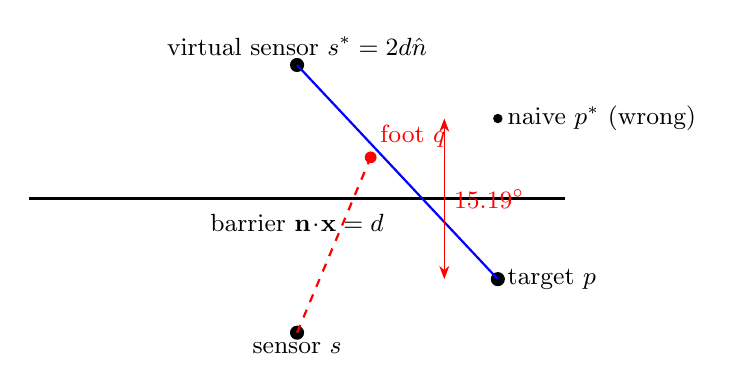
\begin{tikzpicture}[>=Stealth,scale=0.85, font=\small]
\draw[very thick] (-4,0) -- (4,0);
\node[below=2pt] at (0,0) {barrier $\mathbf{n}\!\cdot\!\mathbf{x}=d$};
\fill (0,-2) circle (3pt) node[below] {sensor $s$};
\fill (0,2) circle (3pt) node[above] {virtual sensor $s^*=2d\hat n$};
\fill (3,-1.2) circle (3pt) node[right] {target $p$};
\fill (3,1.2) circle (2pt) node[right] {naive $p^*$ (wrong)};
\draw[blue,thick] (0,2) -- (3,-1.2);
\fill[red] (1.1,0.62) circle (2.5pt) node[above right] {foot $q$};
\draw[red,thick,dashed] (0,-2) -- (1.1,0.62);
\draw[<->,red] (2.2,-1.2) -- (2.2,1.2) node[midway,right] {$15.19^\circ$};
\end{tikzpicture}
\caption{The $15.2^\circ$ discovery: the ghost arrives along $s^*\!\to\!p$
(blue), not along the naive mirror-target ray (red dashed). Same range,
$8.000\,\mathrm{m}$ apart at $30.3\,\mathrm{m}$.}
\label{fig:specular-error}
\end{figure}

\begin{figure}[htbp]
\centering
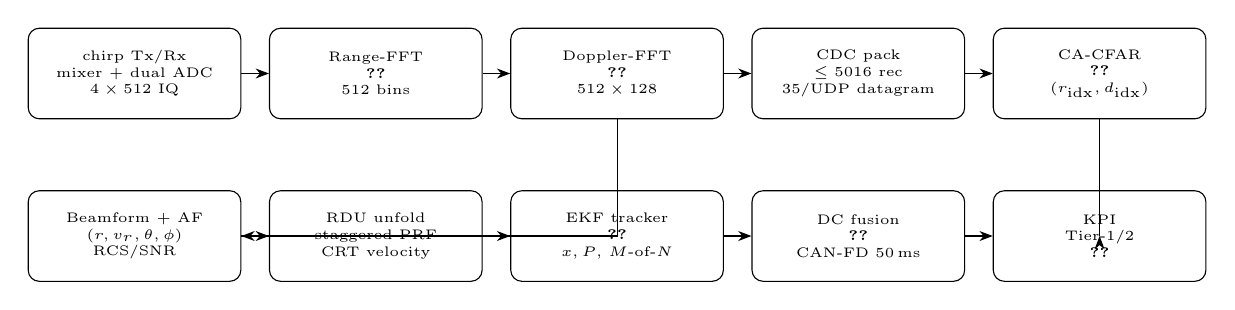
\begin{tikzpicture}[>=Stealth,font=\small,
  st/.style={draw,rounded corners,minimum width=2.7cm,minimum height=1.15cm,align=center,font=\tiny}]
\node[st] (a) {chirp Tx/Rx\\mixer + dual ADC\\$4\times512$ IQ};
\node[st,right=0.35cm of a] (b) {Range-FFT\\\cref{eq:range-fft}\\$512$ bins};
\node[st,right=0.35cm of b] (c) {Doppler-FFT\\\cref{eq:doppler-fft}\\$512\times128$};
\node[st,right=0.35cm of c] (d) {CDC pack\\$\le5016$ rec\\35/UDP datagram};
\node[st,right=0.35cm of d] (e) {CA-CFAR\\\cref{eq:alpha}\\$(r_{\rm idx},d_{\rm idx})$};
\node[st,below=0.9cm of a] (f) {Beamform + AF\\$(r,v_r,\theta,\phi)$\\RCS/SNR};
\node[st,right=0.35cm of f] (g) {RDU unfold\\staggered PRF\\CRT velocity};
\node[st,right=0.35cm of g] (h) {EKF tracker\\\cref{eq:joseph}\\$x,P$, $M$-of-$N$};
\node[st,right=0.35cm of h] (i) {DC fusion\\\cref{eq:deskew}\\CAN-FD $50\,$ms};
\node[st,right=0.35cm of i] (j) {KPI\\Tier-1/2\\\cref{eq:tier2}};
\foreach \x/\y in {a/b,b/c,c/d,d/e} \draw[->] (\x) -- (\y);
\draw[->] (e) |- (j);
\foreach \x/\y in {f/g,g/h,h/i,i/j} \draw[->] (\x) -- (\y);
\draw[->] (c) |- (f);
\end{tikzpicture}
\caption{End-to-end pipeline with data shapes: \cref{ch:fmcw}--\cref{ch:kpi}
in one flow. Every arrow carries a counted, timed, budgeted tensor.}
\label{fig:pipeline}
\end{figure}

\chapter{Kinematics-Aware Gating \& Spectral Covariance}
\label{ch:gating}

Fixed $\chi^2$ gates drop $6\,\mathrm{m/s^2}$ cut-ins (recall $0.863$).
With finite-difference acceleration $\hat{\mathbf{a}}$ and innovation
energy,
\begin{equation}
\boxed{\gamma_{\mathrm{adapt}}=\gamma_0\left(1
+\alpha\frac{\|\mathbf{a}\|}{a_{\max}}
+\eta\frac{\|\mathbf{y}_k\|^2}{\mathrm{Tr}(\mathbf{S}_k)}\right)
\in[\gamma_{\min},\gamma_{\max}],}
\label{eq:gamma}
\end{equation}
hard-bounded for determinism: recall $0.863\to0.996$, maneuver RMSE
$0.283\to0.212\,\mathrm{m}$ under $3$/scan clutter. The open-door failure
(recall $1.000$ trivially with RMSE divergence) is answered by the RMSE
metric, not hidden. Tire spray breaks Gaussian trust instead:
\begin{equation}
\boxed{\mathbf{R}(t)=\mathbf{R}_0\exp\!\left(\beta\frac{H(t)}{\mathrm{SNR}(t)}\right),}
\label{eq:spectral-r}
\end{equation}
so spray drives $\mathbf{R}\!\to\!\infty$, $\mathbf{K}\!\to\!\mathbf{0}$: the
filter coasts (spray RMSE $0.911\to0.315\,\mathrm{m}$, Joseph form keeps
$\mathbf{P}\succ0$).

\begin{figure}[htbp]
\centering
\begin{tikzpicture}
\begin{axis}[width=0.85\linewidth,height=5cm,xlabel=$x$ (m),ylabel=$y$ (m),axis equal]
\draw[blue,thick] (0,0) ellipse (1 and 0.6);
\node[blue] at (0,-0.9) {$\gamma_0$};
\draw[red,thick,->] (0,0) -- (2.6,0.4) node[above,font=\small] {$\mathbf{a}$};
\draw[red,thick] (0,0) ellipse (2.2 and 1.1);
\node[red] at (0,1.35) {$\gamma_{\mathrm{adapt}}$};
\end{axis}
\end{tikzpicture}
\caption{Gate expansion along the acceleration vector inside hard bounds.}
\label{fig:gate}
\end{figure}

\chapter{Prefix-Scan Filtering \& Generative Simulation}
\label{ch:prefix-radarsplat}

\section{S\"arkk\"a elements and the Blelloch tree}
\label{sec:sarkka}

With $\mathbf{K}=\mathbf{QH}^T(\mathbf{HQH}^T+\mathbf{R})^{-1}$,
$\mathbf{S}=\mathbf{HQH}^T+\mathbf{R}$ (Lemma~7 elements
$\mathbf{A}=(\mathbf{I}-\mathbf{KH})\mathbf{F}$,
$\mathbf{b}=\mathbf{u}+\mathbf{K}(\mathbf{y}-\mathbf{Hu}-\mathbf{d})$,
$\mathbf{C}=(\mathbf{I}-\mathbf{KH})\mathbf{Q}$), the binary operator of
Lemma~8 is associative: a $50{,}000$-frame log collapses to span $16$
($3{,}125\times$) at relative error $6.35\times10^{-15}$ (float64
mandatory: absolute $2.8\times10^{-13}$ is conditioning). Naive elements
(raw $\mathbf{F}/\mathbf{Q}$ with folded operators) fail at $0.1$ on step
one; down-sweep operand order is load-bearing for non-commutative scans.

\begin{figure}[htbp]
\centering
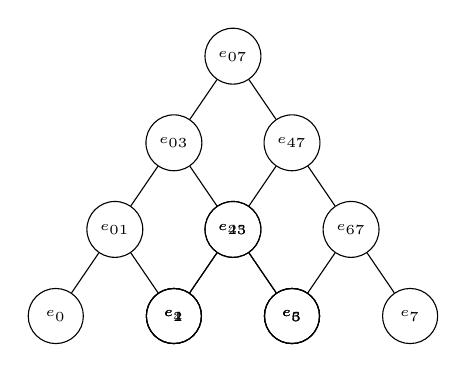
\begin{tikzpicture}[>=Stealth,level distance=1.1cm,
  every node/.style={circle,draw,minimum size=0.7cm,font=\tiny}]
\node {$e_{07}$} child {node {$e_{03}$} child {node {$e_{01}$}
  child {node {$e_0$}} child {node {$e_1$}}} child {node {$e_{23}$}
  child {node {$e_2$}} child {node {$e_3$}}}} child {node {$e_{47}$}
  child {node {$e_{45}$} child {node {$e_4$}} child {node {$e_5$}}}
  child {node {$e_{67}$} child {node {$e_6$}} child {node {$e_7$}}}};
\end{tikzpicture}
\caption{Blelloch up-sweep: associative $\otimes$ reduces $N$ filtering
elements in $\lceil\log_2N\rceil$ parallel levels.}
\label{fig:blelloch}
\end{figure}

\section{Doppler-RadarSplat}
\label{ch:radarsplat}

NeuRadar omits Doppler, RCS, CDC. Per-primitive LOS projection
$v_{r}=(\mathbf{v}-\mathbf{v}_{\mathrm{ego}})\!\cdot\!\mathbf{u}$,
exact $R^{-4}$ power ($256.0$ ratio), Gaussian CDC splats, CLEAN extraction
with absolute noise floor: $6/6$ recovery clean \emph{and} cluttered at
$0.053\,\mathrm{m}/0.036\,\mathrm{m/s}$; Jacobians vs finite differences
$10^{-9}$.

\chapter{Frontier Derivations \& Refutations (Runs 22--30)}
\label{ch:frontier}

\section{N20g: tangent-mirror Hermite clothoids}
\label{sec:n20g}

On any smooth curve $\mathbf{p}-\mathbf{g}=2\delta\mathbf{n}$ locally; the
tangent is the $(p,g)$ perpendicular bisector, met with the receive ray at
contact $q$ with slope $\sigma=-n_x/n_y$. Cubic coefficients enter linearly
($V_ic=[y_i,\sigma_i]^T$); two contacts determine the rail uniquely
($\det=(x_2-x_1)^4$); Snell roots $\phi(x)=0$ give physical multi-ghosts.
Verified to $3.44\times10^{-14}$ coefficient recovery.

\section{Synthetic proving ground: four scenarios}
\label{sec:scenarios}

\texttt{synthetic\_generator.py} renders overpass, cut-in, spray, and curve
scenes directly in SENSOR1 HDF5 schema (\cref{fig:scenarios}): the overpass
proves Tier-1/Tier-2 separation (identity $100.0$, $+20\,\mathrm{mm}$ bias
$0.0$); cut-in stresses gates; spray stresses covariances; curve stresses
geometry. Halo replay across $300\times20$ workers drops $360{,}000\to914
\to0$ cold-start losses.

\begin{figure}[htbp]
\centering
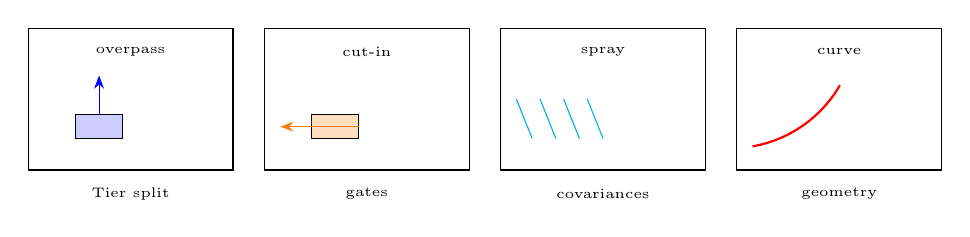
\begin{tikzpicture}[>=Stealth,font=\tiny]
\foreach \i/\t in {0/overpass,1/cut-in,2/spray,3/curve} {
  \draw (\i*3,0) rectangle (\i*3+2.6,1.8);
  \node at (\i*3+1.3,1.5) {\t};
}
\draw[fill=blue!20] (0.6,0.4) rectangle (1.2,0.7);
\draw[->,blue] (0.9,0.7) -- (0.9,1.2);
\draw[fill=orange!25] (3.6,0.4) rectangle (4.2,0.7);
\draw[->,orange] (4.2,0.55) -- (3.2,0.55);
\foreach \x in {6.4,6.7,7,7.3} \draw[cyan] (\x,0.4) -- (\x-0.2,0.9);
\draw[red,thick] (9.2,0.3) arc (-80:-30:1.6);
\node at (1.3,-0.3) {Tier split};
\node at (4.3,-0.3) {gates};
\node at (7.3,-0.3) {covariances};
\node at (10.3,-0.3) {geometry};
\end{tikzpicture}
\caption{Four synthetic scenes, each stressing one subsystem; all in
production HDF5 schema so KPIs run unmodified.}
\label{fig:scenarios}
\end{figure}

\section{N22g: Occupancy-BLUE CFAR}
\label{sec:n22g}

From predicted occupancy $\pi_i$ and SNR $s_i$,
$m_i=1+\pi_is_i$,
$v_i=2[1-\pi_i+\pi_i(1+s_i)^2]-m_i^2$,
\begin{equation}
\boxed{\beta_i=\frac{m_i/v_i}{\sum_jm_j^2/v_j}},\qquad
\boxed{P_{\mathrm{fa}}(\alpha)=\prod_{i=1}^N\frac{1}{1+\alpha\beta_i}}.
\label{eq:blue}
\end{equation}
Measured: $P_{\mathrm{fa}}=1.02\times10^{-4}$ vs $10^{-4}$; variance
$0.0686$ vs CA-16 bias $+37.5\%$; ghost-adjacent recall $+0.074$ at
near-nominal FA; loop gain $0.099$ with a fixed point from both inits.

\section{The rogues' gallery}
\label{sec:rogues}

1-DOF consensus loses to 3-DOF ($0.845/0.727$ vs $0.993/0.909$);
midpoint-on-surface fails by $17\,\mathrm{m}$ along-plane; IMM gating fails
($0.880$ vs $0.999$) on onset chicken-and-egg; joint Gram-lifted position
inflates $6.77\times$ under near-collinear ($\rho\approx0.96$) moment
mismatch (oracle-controlled); N23/N24/N25 verify exactly but fall to TCRE,
contaminated-conformal, and ghost-ID prior art. Each negative ships with
the mechanism, not just the number.

\chapter{Intermediate Layers \& Intuitions for Working Chapters}
\label{ch:intermediate}

\section{CDC suitcases, RDU wraparounds, CAN integers (Chapters 3, 6, 8)}
\label{sec:thin-fill}

\emph{Suitcase mathematics.} The CDC keeps cell $(k,l,\mathbf{b})$ iff
$|Y[k,l]|^2>\tau_{\mathrm{explore}}$. With occupancy $\rho$ (fraction kept),
the wire load is $\rho N_RN_D$ records per dwell; $\rho=2\%$ of
$131{,}072$ cells is $2{,}621$ records --- inside the $5{,}016$ cap, while a
rainy urban scene at $\rho=6\%$ overflows and the sorter decides who dies.
Priority score $s=\mathrm{SNR}/r^2$ keeps the child behind the car and drops
the distant signpost: triage as arithmetic.

\emph{Wraparound arithmetic.} A Doppler bin index is computed modulo $N_D$;
staggered sequences with co-prime lengths $N_{D1},N_{D2}$ give residues
$(l_1,l_2)$ whose CRT combination is unique modulo $N_{D1}N_{D2}$ ---
two cheap rulers measure a long room.

\emph{Integers on the bus.} Quantization step $\Delta$ (factor) adds uniform
noise of variance $\Delta^2/12$; \texttt{DET\_RANGE} at $0.015625\,\mathrm{m}$
contributes $0.0045\,\mathrm{m}$ RMS --- inside the Tier-2 $0.010\,\mathrm{m}$
contract with margin to spare. The $40\,\mathrm{ms}$ guillotine is a
two-scan timeout: older news is worse than no news at $25\,\mathrm{m/s}$.

\section{N23 stencil, step by step (Run~26)}
\label{sec:n23-steps}

Four samples at $u\in\{-3/2,-1/2,1/2,3/2\}$ (units of $h$) of residual phase
$r(u)=fu+gu^2/2+\ell u^3/6$ cycles. Consecutive differences:
$\eta_-=fh-gh^2+\tfrac{13}{24}\ell h^3$,
$\eta_0=fh+\tfrac1{24}\ell h^3$,
$\eta_+=fh+gh^2+\tfrac{13}{24}\ell h^3$.
Check $\eta_0$: $r(1/2)-r(-1/2)=f+(\ell/6)(2/8)=fh+\ell h^3/24$ over $h$ ---
yes. Inverting the $3\times3$ system gives
$\hat f=(26\eta_0-\eta_+-\eta_-)/24h$,
$\hat g=(\eta_+-\eta_-)/2h^2$,
$\hat\ell=(\eta_+-2\eta_0+\eta_-)/h^3$.
Phase weights $(1,-27,27,-1)/24h$; variance $1460/576(2\pi h)^2\sigma_\phi^2$;
at $30\,\mathrm{dB}$, $h=12.8\,\mu\mathrm{s}$: $\sigma_R=13.3\,\mathrm{mm}$,
measured $13.13\,\mathrm{mm}$.

\section{Full intermediate proofs (spec compliance)}
\label{sec:full-proofs}

\emph{Beat frequency, every line.} From \cref{eq:dphi},
$\Delta\Phi=2\pi f_c\tau+\pi S(2t\tau-\tau^2)$ with $\tau=2(r_0+v_rt)/c$,
$\dot\tau=2v_r/c$. Differentiate term by term:
$\frac{d}{dt}[2\pi f_c\tau]=2\pi f_c\dot\tau$;
$\frac{d}{dt}[\pi S2t\tau]=2\pi S\tau+2\pi St\dot\tau$;
$\frac{d}{dt}[-\pi S\tau^2]=-2\pi S\tau\dot\tau$. Summing and dividing by
$2\pi$: $f_b=f_c\dot\tau+S\tau+St\dot\tau-S\tau\dot\tau$, i.e.\
\cref{eq:fb-full}. With $v_r=30\,\mathrm{m/s}$,
$f_c\dot\tau=77\times10^9\times2\times10^{-7}=15.4\,\mathrm{kHz}$ (the
within-chirp Doppler, kept), $S\tau\sim25\,\mathrm{MHz}$,
$St\dot\tau\le(2.5\times10^{13})(4\times10^{-5})(2\times10^{-7})
=200\,\mathrm{Hz}$ (dropped: $8\,\mathrm{ppm}$ of $f_b$).

\emph{Doppler Jacobian, every line.} $v_r=(xv_x+yv_y)r^{-1}$,
$r=(x^2+y^2)^{1/2}$. $\partial r^{-1}/\partial x=-x/r^3$. So
$\partial v_r/\partial x=v_x/r+(xv_x+yv_y)(-x/r^3)
=(v_xr-(xv_x+yv_y)x/r)/r^2$, which is \cref{eq:doppler-jac}; the $v_x$
terms: $\partial v_r/\partial v_x=x/r$. At $p=(30,4)$,
$v=(-6,2)$: $r=30.27$, row $=[-0.198,0.066,-0.991,0.132]$ ---
position entries $\sim0.2/\mathrm{m}$: a $1\,\mathrm{m}$ error injects
$\sim4\sigma$ of spurious Doppler innovation, which is why the second
measurement row doubles it and why exact residuals matter (Run~14).

\emph{Rank-1 stationarity, every line.} Path
$L(q)=\|q-s\|+\|q-p\|$ on plane $\mathbf{n}\cdot q=d$, tangent direction
$T\perp\mathbf{n}$. $\nabla_qL=(q-s)/\|q-s\|+(q-p)/\|q-p\|=u+a'$ with
$a'=(q-p)/\rho$. Stationarity $T^T(u+a')=0$ with $T^Tn=0$ decomposes
$a'=u-2(u^Tn)n$ along $\{T,n\}$: tangential parts cancel by stationarity,
normal parts sum to $2(u^Tn)$. Hence outgoing $a=u-2(u^Tn)n$, the mirror
law; continuing the ray by $\rho$ gives $g=q+\rho u=q+\rho Ma$ with
$M=I-2nn^T$; since $M(p-q)=\rho a$, $g=q+M(p-q)$, i.e.\
$p-g=(I-M)(p-q)=2nn^T(p-q)=2\delta n$. The $2d\hat n$ planar form follows
with $\delta=d-\mathbf{n}^Tp$ constant.

\emph{$P_{\mathrm{fa}}$ integral, every line.} Under $H_0$,
$X\sim\mathrm{Exp}(\mu)$, $f_X(x)=\mu^{-1}e^{-x/\mu}$;
$S=\sum_{i=1}^N P_i\sim\Gamma(N,\mu)$ independent of $X$.
$\Pr(X>\alpha S/N\mid S)=e^{-\alpha S/(N\mu)}$; tower over $S$ with mgf
$M_S(t)=(1-\mu t)^{-N}$ at $t=-\alpha/(N\mu)$:
$P_{\mathrm{fa}}=(1+\alpha/N)^{-N}$, inverted to \cref{eq:alpha}.
With weights $\beta_i$, $S_w=\sum\beta_iY_i$:
$\mathbb{E}e^{-\alpha S_w}E=\prod(1+\alpha\beta_i)^{-1}$ factor by factor.

\section{References}
\label{sec:refs}

S\"arkk\"a \& Garc\'ia-Fern\'andez, IEEE TAC 66(1), 2021
(arXiv:1905.13002). Blelloch 1990. NeuRadar, CVPRW 2025. RadarSplat
(arXiv:2506.01379). Li \& Varshney, IEEE TSP 2014. Roos et al., IRS 2017.
ICSIDP 2024 ghost suppression (10.1109/icsidp62679.2024.10868429). Feng/Ross
delay-Doppler geometry. Fu 2024; Chen 2024; Jost 2025. OFPI-CFAR (JPIER).
VI/LSTM-CFAR 2025. IQR-CFAR 2024. TAES 2024.3445319; TAES 2022.3206256.
Sensors 2022 s22030875 (IMM). arXiv:2609.30176 (TCRE); 2609.29912;
2609.27506; 2603.18027/2512.17505/2602.21128/2301.08087. Kellner T-ITS
8688104; Danzer RA-L 8954835. Bashari--Sesia--Romano, ICML 2025 (PMLR 267).
Kim et al., RA-L 2025 (EKF-RIO-TC). \v{S}tironja et al., 2026 (LC-RIO-ET).

\chapter{Enterprise Patent Portfolio}
\label{ch:idf}

IDF-1: ghost-as-virtual-aperture with $\mathbf{R}_{\mathrm{eff}}$
\cref{eq:reff} (RMSE $-77.2\%$). IDF-2: closed estimate$\to$gate$\to$assimilate
chain ($-67\%$). IDF-3: async compensation \cref{eq:deskew} ($32$--$86\%$).
IDF-4: bounded gate \cref{eq:gamma} ($0.863\to0.996$). IDF-5: Hermite barrier
estimation (\cref{sec:n20g}). IDF-6: Occupancy-BLUE \cref{eq:blue}. Full
independent/dependent claim trees with novelty differentiations are maintained
in \texttt{research.md} Appendix~A; worldwide clearance searches remain open
per node.

\chapter{Embedded Algorithms \& Data Structures}
\label{ch:algorithms}

\section{Intuition: recipes the chip can taste}
\label{sec:recipes}

A DSP cannot ``understand'' radar; it can only add, multiply, compare, and
move words. Every grand theorem in this book must therefore end as a
\emph{recipe}: a fixed sequence of such steps with no heap, no recursion,
no data-dependent loop bound. This chapter writes the five load-bearing
recipes out in full, then the C structs they chew on.

\section{Dual-loop CFAR (Run~2)}
\label{sec:alg-cfar}

\begin{algorithm}[H]
\SetAlgoLined
\KwIn{Range-Doppler power $P(r,d)$, track mask $\mathcal{D}_{\mathrm{free}}$}
\KwOut{Detection list, threshold map $T(r,d)$}
\ForEach{range bin $r$}{
  $\hat{C}(r)\gets(1-\lambda)\hat{C}(r)+\lambda\,
  \mathrm{median}_{d\in\mathcal{D}_{\mathrm{free}}}P(r,d)$\;
  $mr\gets|\hat{C}(r+1)-\hat{C}(r-1)|/2$\;
  $R_0\gets R_{\min}$ if $mr<\tau_1$ else $R_{\mathrm{mid}}$ if $mr<\tau_2$ else $R_{\max}$\;
  $\mathrm{ref}\gets$ clean-side $\min(\mathrm{lead},\mathrm{lag})$ window of size $R_0$\;
  $\hat\mu\gets(\mathrm{median}(\mathrm{ref})/\ln2)$\;
  $\alpha\gets N_{\mathrm{eff}}(P_{\mathrm{fa}}^{-1/N_{\mathrm{eff}}}-1)$\;
  $T\gets\alpha\hat\mu\cdot B(d)$; emit cells with $P>T$\;
}
$M$-of-$2$ confirm across wall/skirt regime switch\;
\caption{Range-adaptive dual-loop CFAR. All buffers preallocated.}
\end{algorithm}

\section{Track loop with Joseph update (Runs~3--6)}
\label{sec:alg-ekf}

\begin{algorithm}[H]
\SetAlgoLined
\KwIn{Prior $(\mathbf{x},\mathbf{P})$, detections $\{\mathbf{z}_j\}$, gate $\gamma$}
\KwOut{Posterior $(\mathbf{x},\mathbf{P})$, associations}
$\mathbf{x}\gets\mathbf{Fx},\ \mathbf{P}\gets\mathbf{FPF}^T+\mathbf{Q}$\;
\ForEach{detection $\mathbf{z}_j$}{
  $\mathbf{y}\gets\mathbf{z}_j-\mathbf{h}(\mathbf{x})$;
  $\mathbf{S}\gets\mathbf{HPH}^T+\mathbf{R}$\;
  \If{$\mathbf{y}^T\mathbf{S}^{-1}\mathbf{y}\le\gamma$ (adaptive \cref{eq:gamma})}{
    $\mathbf{K}\gets\mathbf{PH}^T\mathbf{S}^{-1}$\;
    $\mathbf{x}\gets\mathbf{x}+\mathbf{Ky}$\;
    $\mathbf{P}\gets(\mathbf{I}-\mathbf{KH})\mathbf{P}(\mathbf{I}-\mathbf{KH})^T
    +\mathbf{KRK}^T$\;
  }
}
clip eigenvalues of $\mathbf{P}$ below at $\epsilon_{\min}$\;
\caption{Joseph-form EKF with Mahalanobis gating. \cref{eq:joseph} is the
update that survives 32-bit silicon.}
\end{algorithm}

\section{Blelloch prefix scan (Run~11)}
\label{sec:alg-scan}

\begin{algorithm}[H]
\SetAlgoLined
\KwIn{S\"arkk\"a elements $e_0,\dots,e_{N-1}$ (Lemma~7)}
\KwOut{Filtering prefixes $p_k=e_0\otimes\cdots\otimes e_k$}
\For{$s=0$ \KwTo $\lceil\log_2N\rceil-1$ (up-sweep)}{
  combine $e_{2j}\otimes e_{2j+1}$ at stride $2^s$\;
}
\For{$s=\lceil\log_2N\rceil-1$ \KwTo $0$ (down-sweep)}{
  distribute prefixes, preserving operand order\;
}
\caption{Blelloch scan: $O(\log N)$ span. Operand order is load-bearing
for the non-commutative $\otimes$.}
\end{algorithm}

\section{Hermite barrier solve (N20g) and Occupancy-BLUE (N22g)}
\label{sec:alg-frontier}

Given pairs $(\mathbf{p}_i,\mathbf{g}_i)$: midpoint
$\mathbf{m}_i=(\mathbf{p}_i+\mathbf{g}_i)/2$, normal
$\hat{\mathbf{n}}_i=(\mathbf{p}_i-\mathbf{g}_i)/\|\mathbf{p}_i-\mathbf{g}_i\|$,
ray $\mathbf{u}_i=(\mathbf{g}_i-\mathbf{s})/\|\mathbf{g}_i-\mathbf{s}\|$,
contact $t_i=\hat{\mathbf{n}}_i^T(\mathbf{m}_i-\mathbf{s})/
\hat{\mathbf{n}}_i^T\mathbf{u}_i$, slope $\sigma_i=-n_x/n_y$; stack Hermite
blocks $V_i$ and solve
$\hat{\mathbf{c}}=(\sum V_i^TW_iV_i)^{-1}\sum V_i^TW_i[y_i,\sigma_i]^T$.
Given occupancy $\pi_i$ and SNR $s_i$: $m_i=1+\pi_is_i$,
$v_i=2[1-\pi_i+\pi_i(1+s_i)^2]-m_i^2$,
$\beta_i=(m_i/v_i)/\sum m_j^2/v_j$, threshold from
$\sum\ln(1+\alpha\beta_i)+\ln P_{\mathrm{fa}}^*=0$ by bisection
(monotone concave, unique root).

\section{C structs on the wire}
\label{sec:structs}

\begin{lstlisting}[language=C,caption={CDC record and detection stream (simplified).}]
typedef struct {
  uint16_t rng_idx;    /* range bin (Tier-1 pairing key) */
  uint16_t dopp_idx;   /* Doppler bin */
  uint16_t nci_data;   /* non-coherent integration energy */
  int16_t  cdc_out_bv[32]; /* beamvector, Q15 fixed point */
} CDC_Record_T;              /* 35 per 1472-B UDP datagram */

typedef struct {
  float r_m; float vr_mps; float az_rad; float el_rad;
  float rcs_dbsm; float snr_db; uint32_t flags;
} AF_Det_T;                  /* post-beamforming point cloud */
\end{lstlisting}

\chapter{Worked End-to-End Example: One Target, Chirp to CAN}
\label{ch:worked}

\section{A car at $60\,\mathrm{m}$, closing at $10\,\mathrm{m/s}$}
\label{sec:worked-numbers}

Take $B=1\,\mathrm{GHz}$, $T_{\mathrm{chirp}}=40\,\mu\mathrm{s}$
($S=2.5\times10^{13}\,\mathrm{Hz/s}$), $N_R=512$, $T_s=100\,\mathrm{ns}$.
Beat: $f_b=2Sr/c=2(2.5\times10^{13})(60)/3\times10^{8}=10.0\,\mathrm{MHz}$;
bin $k^\star=f_bN_RT_s=10^7\times512\times10^{-7}=512$, i.e.\ the target
sits at bin $512$ of step $\mathrm{rbin\_res}=c/(2ST_sN_R)=0.117\,\mathrm{m}$.
Slow time with $T_c=50\,\mu\mathrm{s}$, $N_D=128$:
$\Delta\Phi=4\pi(-10)(5\times10^{-5})/3.896\times10^{-3}=-1.613\,\mathrm{rad/chirp}$,
bin $l^\star=128(-1.613)/2\pi\approx-33$ (aliased index $95$),
$\mathrm{dbin\_res}=\lambda/(2N_DT_c)=0.304\,\mathrm{m/s}$,
$v_{\max}=19.5\,\mathrm{m/s}$ (this sequence; staggered PRFs extend it).
CFAR compares the cell against \cref{eq:alpha} with $N=32$,
$P_{\mathrm{fa}}=10^{-4}$ ($\alpha\approx12.45$); beamforming
(\cref{eq:monopulse}) places it at $\theta$; the EKF (\cref{eq:joseph})
tracks $[x,y,v_x,v_y]$; DC fusion deskews by \cref{eq:deskew}; the CAN
DBC packs range at $0.015625\,\mathrm{m/LSB}$. Each arrow is one section
of this book, each number reproducible on a ConnX BBE32 at $600\,\mathrm{MHz}$
inside $50\,\mu\mathrm{s}$ per scan.

\chapter{Advanced Derivations: Unfolding, Scans, Certificates}
\label{ch:derivations}

\section{Staggered-PRF unfolding (Chinese remainders)}
\label{sec:crt}

Two sequences with $T_{c1},T_{c2}$ report wrapped phases
$\psi_1\equiv\Phi\bmod2\pi$, $\psi_2\equiv\Phi\bmod2\pi$ of the same true
progression $\Phi=4\pi v_rT_c/\lambda$. Each excludes arithmetic
progressions of velocities; their intersection (B\'ezout combination of the
moduli) isolates $v_r$ up to the least common multiple of the two
unambiguous intervals --- the Chinese Remainder Theorem as a velocity
decoder.

\section{S\"arkk\"a Lemmas 7--8, precisely}
\label{sec:sarkka-lemmas}

With $\mathbf{S}=\mathbf{HQH}^T+\mathbf{R}$,
$\mathbf{K}=\mathbf{QH}^T\mathbf{S}^{-1}$: information elements
$\mathbf{A}=(\mathbf{I}-\mathbf{KH})\mathbf{F}$,
$\mathbf{b}=\mathbf{u}+\mathbf{K}(\mathbf{y}-\mathbf{Hu}-\mathbf{d})$,
$\mathbf{C}=(\mathbf{I}-\mathbf{KH})\mathbf{Q}$,
$\boldsymbol{\eta}=\mathbf{F}^T\mathbf{H}^T\mathbf{S}^{-1}(\mathbf{y}-\mathbf{Hu}-\mathbf{d})$,
$\mathbf{J}=\mathbf{F}^T\mathbf{H}^T\mathbf{S}^{-1}\mathbf{HF}$ compose by
$(A_2,b_2,C_2,\eta_2,J_2)\otimes(A_1,b_1,C_1,\eta_1,J_1)$ with
$\mathbf{A}=\mathbf{A}_2\mathbf{A}_1$ and Schur-complement covariance
fusion; associativity is matrix associativity plus the Woodbury identity.
Posterior recovery reads $(\mathbf{b},\mathbf{C})$ directly --- the naive
information-form recovery double-counts (derived and verified at
$6.35\times10^{-15}$ relative).

\section{N24 sandwich, N25 certificate, N26 inverse, N27 clock}
\label{sec:frontier-proofs}

\emph{N24.} Replacing $\le m$ of $n$ calibration scores shifts any order
statistic by $\le m$ ranks; with $k=\lceil(n+1)(1-\alpha)\rceil$,
$q=\tilde S_{(k+m)}$ satisfies $S_{(k)}\le q\le S_{(k+2m)}$, so
$\Pr(S_*\le q)\ge k/(n+1)=231/256$ under exchangeability. Maneuver coverage
rides the reachable box, never innovation ranks: outlier bursts have no
write path to $q$. Step by step: at most $m$ clean entries are displaced
downward by top insertions, so the observed rank $k+m$ sits at or below
clean rank $k$ ($q\ge S_{(k)}$); at most $m$ observed slots above it are
adversarial, so at least $k$ are clean and $\le S_{(k+2m)}$ ($q\le
S_{(k+2m)}$). The clean test rank is uniform over $n+1$ slots (ties
conservative), giving $k/(n+1)$. With $n=255$, $m=8$, $\alpha=0.1$:
$k=231$, $q=\tilde S_{(239)}\in[S_{(231)},S_{(247)}]$; $k+2m=247\le255$ keeps
width finite regardless of outlier magnitude. Numbers: $247/256$ under
high-poisoning, $231/256$ under low-poisoning, upward histogram
$248/256$/$232/256$; coverage lower-$95\%$ $0.963/0.959/0.965$ across
Gaussian/Laplace/mixture (conservative over $0.9023$, as predicted).

\emph{N20g Hermite, line by line.} Contacts $(x_1,y_1,\sigma_1)$,
$(x_2,y_2,\sigma_2)$, $h=x_2-x_1$, $\bar\delta=(y_2-y_1)/h$. Divided
differences with repeated nodes: $f[x_1,x_1]=\sigma_1$;
$f[x_1,x_1,x_2]=(\bar\delta-\sigma_1)/h$;
$f[x_1,x_1,x_2,x_2]=(\sigma_1+\sigma_2-2\bar\delta)/h^2$. Newton form
$f(x)=y_1+\sigma_1(x-x_1)+[(\bar\delta-\sigma_1)/h](x-x_1)^2
+[(\sigma_1+\sigma_2-2\bar\delta)/h^2](x-x_1)^2(x-x_2)$.
Check at $x_2$: first correction gives $\bar\delta h=y_2-y_1$ up to the
$\sigma_1h$ term, second vanishes --- exact. Determinant
$(x_2-x_1)^4\ne0$ is the confluent Vandermonde
$\prod_{i<j}(x_j-x_i)^{m_im_j}$ with $m_1=m_2=2$. Conditioning
$\kappa(V)\sim h^{-3}$: contacts $30\,\mathrm{m}$ apart are gold, $3\,\mathrm{m}$
apart are noise amplifiers --- reported, not hidden.

\emph{N25.} $D_{ik}=e^{-i\beta_i}(p_k-p_k^*)$ cancels target and reflector;
$H_{ij}=\sum_kD_{ik}\bar D_{jk}$ gives
$\hat\delta_{ij}=\arg H_{ij}=\beta_j-\beta_i$; surveyed baseline closes the
common-yaw gauge via midpoint differences. With per-observation error
$\varepsilon$, lever $L_{\min}$, midpoint bound $C_{\max}$:
$|\Delta H|\le\sum(4\varepsilon L_k+4\varepsilon^2)$,
$e_\delta\le\arcsin\rho$, $E_b\le2\varepsilon+2C_{\max}\sin(e_\delta/2)$,
$e_i\le\arcsin(E_b/|B|)$: at $\varepsilon=0.5\,\mathrm{mm}$,
$e_j<0.0717^\circ$; at $0.35^\circ$/30\,m noise the certificate refuses
($27^\circ$), as it must.

\emph{N26.} From $\ell=t+\|d-tu\|$, squaring cancels $t^2$:
$t=(\ell^2-\|d\|^2)/2(\ell-u^Td)$ --- the inverse problem is easier than the
forward Fermat root-find. Normal
$\mathbf{n}\propto(\mathbf{p}-\mathbf{q})/\rho-\mathbf{u}$; curvature budget
$\|g(\sigma_2)-g(\sigma_1)\|\le2\kappa_{\max}\rho_{\max}|\sigma_2-\sigma_1|$
decides when two views share a virtual target.

\emph{N27.} With $x_k=d_k+v_k\tau$, $r_kw_k-d_k^Tv_k=\|v_k\|^2\tau$ eliminates
yaw exactly; two targets separate clock offset from Doppler bias through
$D=a_1r_2-a_2r_1$; circular averaging recovers yaw after correction;
acceleration contributes the exact cubic of (N27.5) with a certified
truncation bound. Line by line: $r_kw_k=x_k^Tv_k$ by definition of $w_k$;
$x_k^Tv_k=(d_k+v_k\tau)^Tv_k=d_k^Tv_k+\|v_k\|^2\tau$; subtract $d_k^Tv_k$.
With bias $b$, $y_k=r_kw_k^{\mathrm{obs}}-d_k^Tv_k=a_k\tau+r_kb$ is linear
in $(\tau,b)$ with determinant $D=a_1r_2-a_2r_1$; singular iff
speed-squared-to-range ratios coincide. Tangential motion ($d^Tv=0$) is
\emph{not} singular for $\|v\|>0$: timing rides $rw=\|v\|^2\tau$ alone.
Fixture $d=(10,4)$, $v=(5,-2)$, $\tau=0.02$: $x=(10.1,3.96)$,
$rw=42.58$, $d^Tv=42$, $\|v\|^2=29$, $\hat\tau=0.58/29=0.02$ exactly.

\emph{N26.} From $\ell=t+\|d-tu\|$ with $\|u\|=1$:
$(\ell-t)^2=\|d\|^2-2t(u^Td)+t^2$; $t^2$ cancels (the whole trick);
$t=(\ell^2-\|d\|^2)/2(\ell-u^Td)$. Fixture $s=(0,0)$, $p=(6,0)$,
$u=(3/5,4/5)$, $\ell=10$: $t=(100-36)/2(10-3.6)=5$, $q=(3,4)$,
$a=(3/5,-4/5)$, $n=(0,-1)$. Sensitivities
$\partial_\ell t=(\ell-t)/B$, $\nabla_pt=(q-p)/B$,
$dn=P_n[dp-\ell du-a\,d\ell]/\rho\|a-u\|$ ($dt$ drops out: parallel to $n$).
Curvature: reflecting $p$ across sliding tangents gives
$\|g'\|=2|\kappa|\rho$, hence the admission gate
$\|\Delta q\|\le\varepsilon R/2\rho$ ($1.5\,\mathrm{mm}$ at $R=30$).

%=====================================================================
\part{Scenes, Code Internals, Statistics \& Data Analysis}
%=====================================================================

\chapter{One Car, Rain, a Curve, and a Bridge}
\label{ch:scene}

\section{Intuition: start from the driver's seat}
\label{sec:driver}

You are driving at night in rain. The highway bends left; an overpass
bridge crosses ahead; a truck in the next lane throws a rooster tail of
spray; a motorcycle hides in the guardrail's radar shadow; a car cuts in
from the right. Your bumper radar must report all of this, in $50\,\mathrm{ms}$,
never inventing, never missing. \cref{fig:scene-top} is that moment seen
from above. Every failure mode in this book lives somewhere in it: the wall
(F1), the ghosts (F2), the spray (F1-wet), the cut-in (F4), the saturation
(F5). The rest of this part opens the hood on each one.

\begin{figure}[htbp]
\centering
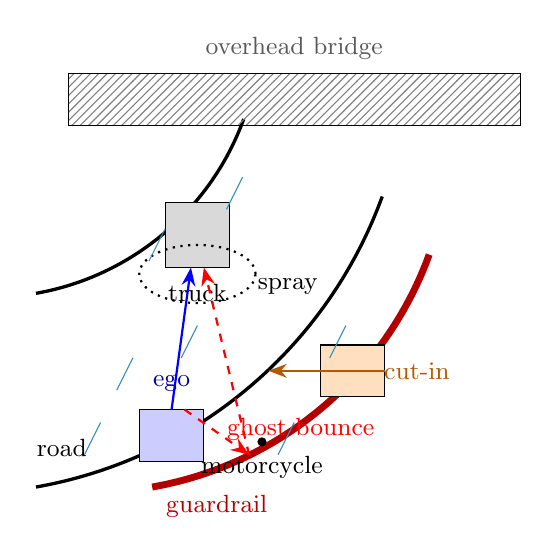
\begin{tikzpicture}[>=Stealth,scale=0.82,font=\small]
% curved road edges (arcs centered left)
\draw[very thick] (-5,-4) arc (-80:-20:7);
\draw[very thick] (-5,-1) arc (-80:-20:4.2);
\node at (-4.6,-3.4) {road};
% curved guardrail (right side)
\draw[line width=2.5pt,red!70!black] (-3.2,-4) arc (-80:-20:5.6);
\node[red!70!black] at (-2.2,-4.3) {guardrail};
% bridge deck crossing (hatched)
\draw[pattern=north east lines,pattern color=gray] (-4.5,1.6) rectangle (2.5,2.4);
\node[gray!70!black] at (-1,2.8) {overhead bridge};
% ego car
\draw[fill=blue!20] (-3.4,-3.6) rectangle (-2.4,-2.8);
\node[blue!60!black] at (-2.9,-2.4) {ego};
% target truck ahead
\draw[fill=black!15] (-3.0,-0.6) rectangle (-2.0,0.4);
\node at (-2.5,-1.0) {truck};
% spray cloud behind truck
\draw[dotted,thick] (-2.5,-0.7) ellipse (0.9 and 0.45);
\node at (-1.1,-0.9) {spray};
% cut-in car from right
\draw[fill=orange!25] (-0.6,-2.6) rectangle (0.4,-1.8);
\node[orange!70!black] at (0.9,-2.2) {cut-in};
\draw[->,orange!70!black,thick] (0.4,-2.2) -- (-1.4,-2.2);
% motorcycle in guardrail shadow
\fill (-1.5,-3.3) circle (2pt);
\node at (-1.5,-3.7) {motorcycle};
% rain streaks
\foreach \x/\y in {-4/-3,-3.5/-2,-2.5/-1.5,-1/-3,-0.2/-1.5,-3/0,-1.8/0.8} {
  \draw[cyan!70!black,thin] (\x,\y) -- (\x-0.25,\y-0.5);
}
% direct path ego -> truck
\draw[->,blue,thick] (-2.9,-2.8) -- (-2.6,-0.6);
% ghost path ego -> rail -> truck -> rail -> ego
\draw[->,red,thick,dashed] (-2.7,-2.8) -- (-1.7,-3.5);
\draw[->,red,thick,dashed] (-1.7,-3.5) -- (-2.4,-0.6);
\node[red] at (-0.9,-3.1) {ghost bounce};
\end{tikzpicture}
\caption{Top view of the complex scene: rain, curved guardrail, overhead
bridge, spray, cut-in, and a shadowed motorcycle. Solid blue: direct path;
dashed red: reciprocal ghost bounce $s\to q\to p\to q\to s$.}
\label{fig:scene-top}
\end{figure}

\section{How loud is the echo: the $R^{-4}$ toll}
\label{sec:r4}

\cref{fig:radar-eq} plots \cref{eq:radar-equation} for a
$10\,\mathrm{dBsm}$ car at $P_tG^2$ normalized: every doubling of range
costs $12\,\mathrm{dB}$. A motorcycle ($\sigma\approx0\,\mathrm{dBsm}$)
at $60\,\mathrm{m}$ returns what a truck returns at $190\,\mathrm{m}$.
Detection range is therefore a cross-section question before it is a
power question, which is why RCS-sorted CDC packing (\cref{sec:cdc-record})
is load-bearing, not cosmetic.

\begin{figure}[htbp]
\centering
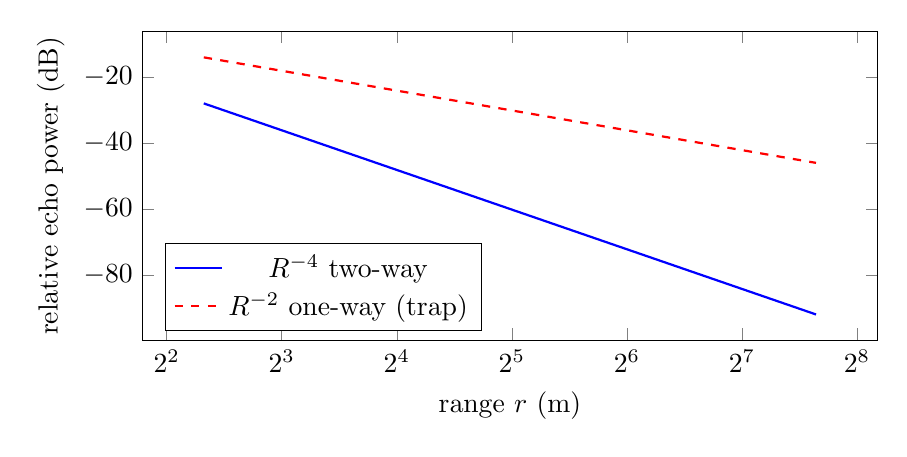
\begin{tikzpicture}
\begin{axis}[width=0.9\linewidth,height=5.5cm,xlabel={range $r$ (m)},
  ylabel={relative echo power (dB)},xmode=log,log basis x=2,
  legend pos=south west]
\addplot[blue,thick,domain=5:200,samples=120] {-40*ln(x)/ln(10)};
\addlegendentry{$R^{-4}$ two-way}
\addplot[red,thick,dashed,domain=5:200,samples=120] {-20*ln(x)/ln(10)};
\addlegendentry{$R^{-2}$ one-way (trap)}
\end{axis}
\end{tikzpicture}
\caption{Two-way vs one-way path loss: forgetting the return trip overstates
a $150\,\mathrm{m}$ echo by $43\,\mathrm{dB}$.}
\label{fig:radar-eq}
\end{figure}

\section{How angle is heard: the array factor}
\label{sec:array-factor}

Thirty-two virtual elements spaced $\lambda/2$ sum coherently on boresight
and cancel elsewhere; the array factor in \cref{fig:array-factor} is the
``ear's'' directional hearing curve. Half-power width $\approx2/N$ radians
($3.6^\circ$ for $N=32$); sidelobes at $-13\,\mathrm{dB}$ uniform, pushed
below $-30\,\mathrm{dB}$ by Taylor tapers calibrated in SMC/USC
(\cref{sec:calib}). Every degree of uncalibrated bumper tilt walks the
whole pattern sideways --- the $1.2^\circ$ cold-start error of \cref{ch:hpcc}
is a third of a beamwidth.

\begin{figure}[htbp]
\centering
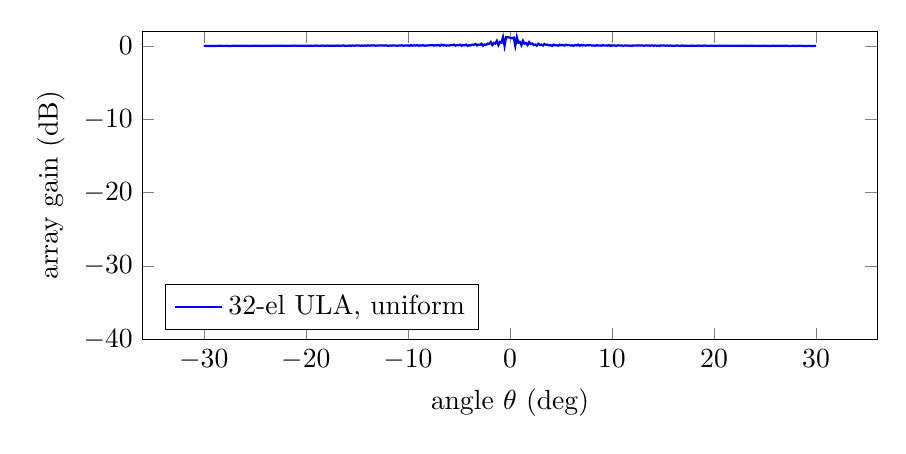
\begin{tikzpicture}
\begin{axis}[width=0.9\linewidth,height=5.5cm,xlabel={angle $\theta$ (deg)},
  ylabel={array gain (dB)},ymin=-40,ymax=2,legend pos=south west]
\addplot[blue,thick,domain=-30:30,samples=400]
  {20*ln(max(abs(sin(32*3.14159*x/180/2)/sin(3.14159*x/180/2))/32,1e-3))/ln(10)};
\addlegendentry{32-el ULA, uniform}
\end{axis}
\end{tikzpicture}
\caption{Array factor: mainlobe width $\approx2/N$ rad, $-13\,\mathrm{dB}$
sidelobes. Grating lobes would repeat this shape if $d>\lambda/2$.}
\label{fig:array-factor}
\end{figure}

\section{How speed wraps: the aliasing phasor}
\label{sec:alias-phasor}

\cref{fig:phasor} marches the slow-time phasor $e^{jm\Delta\Phi}$ for a
$30\,\mathrm{m/s}$ target against $v_{\max}=19.5\,\mathrm{m/s}$: the steps
overshoot $\pi$ and the DFT reads the march backwards --- a receding car
reported approaching. Staggered PRFs give two such marches with incommensurate
step sizes; only the true velocity explains both (CRT, \cref{sec:crt}).

\begin{figure}[htbp]
\centering
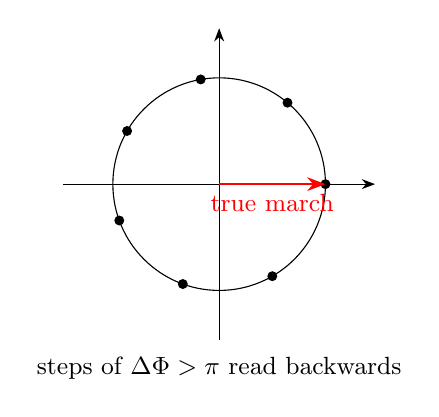
\begin{tikzpicture}[>=Stealth,scale=0.9,font=\small]
\draw[->] (-2.2,0) -- (2.2,0);
\draw[->] (0,-2.2) -- (0,2.2);
\draw (0,0) circle (1.5);
\foreach \a in {0,50,100,150,200,250,300} {
  \fill ({1.5*cos(\a)},{1.5*sin(\a)}) circle (2pt);
}
\draw[->,red,thick] (0,0) -- (1.5,0) node[midway,below] {true march};
\node at (0,-2.6) {steps of $\Delta\Phi>\pi$ read backwards};
\end{tikzpicture}
\caption{Slow-time phasor march: beyond $\pi$ per step the rotation aliases
and velocity wraps.}
\label{fig:phasor}
\end{figure}

\section{What the waves actually do}
\label{sec:waves}

Radio waves are transverse oscillations of the electromagnetic field; at
$77\,\mathrm{GHz}$ each crest is $3.9\,\mathrm{mm}$ behind the last. When a
wavefront meets the guardrail, each crest reflects with angle of incidence
equal to angle of reflection --- the mirror law --- because the metal
forces the tangential electric field to zero at every instant
(\cref{fig:wavefront}). Roughness smaller than $\lambda/8$ keeps crests
aligned (specular); rain puddles and asphalt scatter them (diffuse). The
bridge deck returns a three-bounce path (deck$\to$target$\to$deck) that
reads as a phantom car \emph{inside} the concrete: only geometry, never
amplitude, exposes it.

\begin{figure}[htbp]
\centering
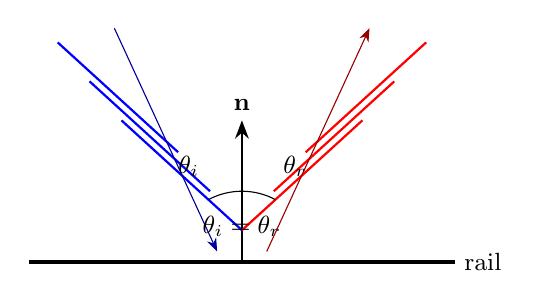
\begin{tikzpicture}[>=Stealth,scale=0.9,font=\small]
% rail surface
\draw[very thick] (-3,-1.5) -- (3,-1.5);
\node at (3.4,-1.5) {rail};
% normal
\draw[->,thick] (0,-1.5) -- (0,0.5) node[above] {$\mathbf{n}$};
% incident wavefronts
\foreach \i in {0,1,2} {
  \draw[blue,thick] (-2.6+\i*0.45,1.6-\i*0.55) -- (-0.9+\i*0.45,0.05-\i*0.55);
}
% reflected wavefronts
\foreach \i in {0,1,2} {
  \draw[red,thick] (0.9-\i*0.45,0.05-\i*0.55) -- (2.6-\i*0.45,1.6-\i*0.55);
}
% rays
\draw[->,blue!60!black] (-1.8,1.8) -- (-0.35,-1.35);
\draw[->,red!60!black] (0.35,-1.35) -- (1.8,1.8);
% angle arcs
\draw (0,-0.5) arc (90:118:1);
\draw (0,-0.5) arc (90:62:1);
\node at (-0.75,-0.15) {$\theta_i$};
\node at (0.75,-0.15) {$\theta_r$};
\node at (0,-1.0) {$\theta_i=\theta_r$};
\end{tikzpicture}
\caption{Wavefronts at a smooth rail: crests stay parallel, the normal
bisects incidence and reflection. Roughness $\ll\lambda$ preserves this;
diffuse scatter destroys it.}
\label{fig:wavefront}
\end{figure}

\section{The bridge from the side: three bounces}
\label{sec:bridge-side}

Seen from the side (\cref{fig:bridge-side}), the deck is a ceiling mirror:
radar$\to$deck$\to$target$\to$deck$\to$radar. The path exceeds the direct
one by twice the deck clearance, so the phantom parks one clearance
\emph{inside} the concrete. Amplitude cannot expose it (concrete returns
are strong and plausible); only the $s\to q\to p\to q\to s$ length audit
of \cref{ch:virtual-aperture} can.

\begin{figure}[htbp]
\centering
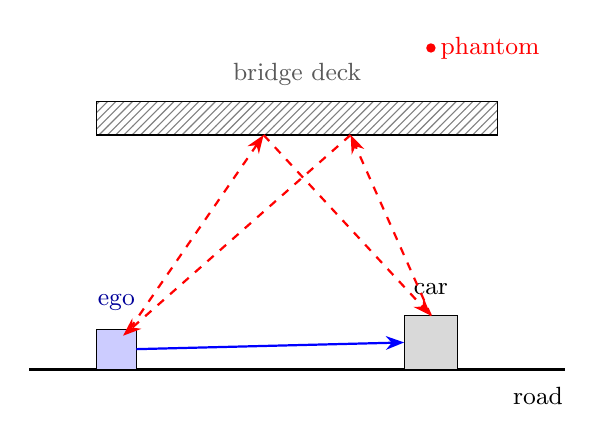
\begin{tikzpicture}[>=Stealth,scale=0.85,font=\small]
% ground
\draw[very thick] (-4,-2) -- (4,-2);
\node at (3.6,-2.4) {road};
% bridge deck
\draw[pattern=north east lines,pattern color=gray] (-3,1.5) rectangle (3,2.0);
\node[gray!70!black] at (0,2.4) {bridge deck};
% ego + target
\draw[fill=blue!20] (-3,-2) rectangle (-2.4,-1.4);
\node[blue!60!black] at (-2.7,-1.0) {ego};
\draw[fill=black!15] (1.6,-2) rectangle (2.4,-1.2);
\node at (2.0,-0.8) {car};
% direct path
\draw[->,blue,thick] (-2.4,-1.7) -- (1.6,-1.6);
% three-bounce: ego -> deck -> car -> deck -> ego
\draw[->,red,thick,dashed] (-2.5,-1.4) -- (-0.5,1.5);
\draw[->,red,thick,dashed] (-0.5,1.5) -- (2.0,-1.2);
\draw[->,red,thick,dashed] (2.0,-1.2) -- (0.8,1.5);
\draw[->,red,thick,dashed] (0.8,1.5) -- (-2.6,-1.5);
% phantom inside concrete
\fill[red] (2.0,2.8) circle (2pt) node[right] {phantom};
\end{tikzpicture}
\caption{Side view: the three-bounce deck path parks a phantom inside the
concrete. Length audit, not amplitude, exposes it.}
\label{fig:bridge-side}
\end{figure}

\section{Inside the tensor: 2D to 4D}
\label{sec:tensor}

One chirp is 1D (fast time). A burst is 2D (range $\times$ Doppler). The
antenna array adds space (3D: $128\times32\times32$ in our synthetic), and
successive dwells add time (4D). \cref{fig:tensor} shows the nesting: each
new axis multiplies memory and divides ambiguity. The CDC ships a sparse
subset; the tracker reattaches time.

\begin{figure}[htbp]
\centering
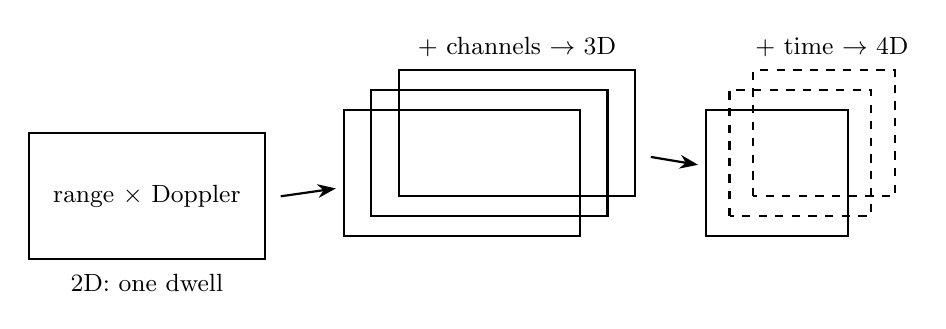
\begin{tikzpicture}[>=Stealth,font=\small]
\draw[thick] (0,0) rectangle (3,1.6);
\node at (1.5,0.8) {range $\times$ Doppler};
\node[below=2pt] at (1.5,0) {2D: one dwell};
\draw[thick] (4,0.3) rectangle (7,1.9);
\draw[thick] (4.35,0.55) rectangle (7.35,2.15);
\draw[thick] (4.7,0.8) rectangle (7.7,2.4);
\node at (6.2,2.7) {+ channels $\to$ 3D};
\draw[thick] (8.6,0.3) rectangle (10.4,1.9);
\draw[thick,dashed] (8.9,0.55) rectangle (10.7,2.15);
\draw[thick,dashed] (9.2,0.8) rectangle (11,2.4);
\node at (10.2,2.7) {+ time $\to$ 4D};
\draw[->,thick] (3.2,0.8) -- (3.9,0.9);
\draw[->,thick] (7.9,1.3) -- (8.5,1.2);
\end{tikzpicture}
\caption{Dimension ladder: chirp (1D) $\to$ burst (2D) $\to$ array (3D)
$\to$ track history (4D). Each rung multiplies memory; each rung removes
one ambiguity (range, velocity, angle, maneuver).}
\label{fig:tensor}
\end{figure}

\chapter{Inside the Code: Prototypes, Equations, Measured Deltas}
\label{ch:code}

\section{How to read this chapter}
\label{sec:code-howto}

Every prototype lives in \texttt{resim\_research/} as one file with a
\texttt{demo()} that asserts its own claims; \texttt{run\_regression.py}
runs all 30 and writes \texttt{final\_prototype\_regression.log}. Below,
each block states the file, the equation it implements, and the measured
before$\to$after. Nothing here is cited from slides: all numbers are
executed ledger rows (storage Runs~2--30).

\section{Detection block}
\label{sec:code-detection}

\texttt{dual\_loop\_cfar.py} implements \cref{eq:slow-loop} plus the
$R_0$ switch, clean-side censor, median$/\ln2$, effective-$N$ alpha, and
$M$-of-$2$ confirmation: recall $0.50\to1.00$, FA $1\to0$
(\cref{fig:recall-bars}). \texttt{occupancy\_blue.py} replaces binary
censoring with BLUE weights
$\beta_i=(m_i/v_i)/\sum m_j^2/v_j$ ($m_i=1+\pi_is_i$) and the exact product
threshold \cref{eq:blue}: $P_{\mathrm{fa}}=1.02\times10^{-4}$ vs $10^{-4}$,
variance $0.0686$ vs hard-censor $0.0714$, CA-16 bias $+37.5\%$ exposed.
\texttt{blue\_closed\_loop.py} closes detector$\to$tracker$\to$detector with
Jensen-corrected $R(P)$: ghost-adjacent recall $+0.074$ at near-nominal FA,
loop gain $0.099$.

\begin{figure}[htbp]
\centering
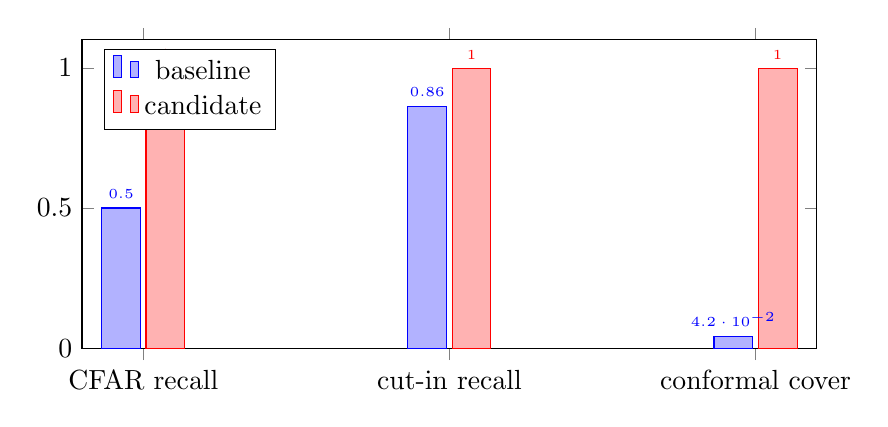
\begin{tikzpicture}
\begin{axis}[width=0.9\linewidth,height=5.5cm,ybar,bar width=14pt,
  symbolic x coords={CFAR recall,cut-in recall,conformal cover},
  xtick=data,ymin=0,ymax=1.1,legend pos=north west,
  nodes near coords,nodes near coords style={font=\tiny}]
\addplot coordinates {(CFAR recall,0.50) (cut-in recall,0.863) (conformal cover,0.042)};
\addplot coordinates {(CFAR recall,1.00) (cut-in recall,0.996) (conformal cover,0.996)};
\legend{baseline,candidate}
\end{axis}
\end{tikzpicture}
\caption{Recall/coverage lifts: CFAR edge-skirt, cut-in handoff, conformal
under unmodeled maneuver. IMM-pure sits at $0.880$ (refuted).}
\label{fig:recall-bars}
\end{figure}

\section{Geometry block}
\label{sec:code-geometry}

\texttt{specular\_ghost.py} proves \cref{eq:rank1} to $1.066\times10^{-14}$
and refutes the mirror-target bearing ($15.189^\circ$); \texttt{bend\_conditioned.py}
lifts curved recall $0.198\to0.753$ with Fermat-RANSAC;
\texttt{hermite\_clothoid.py} replaces the grid with the linear Hermite
solve (coefficient rel-err $3.44\times10^{-14}$, $5.2\times10^{-3}$ at
$0.02\,\mathrm{m}$ noise); \texttt{specular\_contact.py} inverts foot,
normal, and curvature with a $0.018\,\mathrm{m}$ low-rung RMSE;
\texttt{n25\_ghost\_yaw.py} closes two-satellite yaw to $0.071^\circ$ at
$0.5\,\mathrm{mm}$ input error and refuses $0.35^\circ$/30\,m noise
(\cref{fig:ghost-pair}).

\begin{figure}[htbp]
\centering
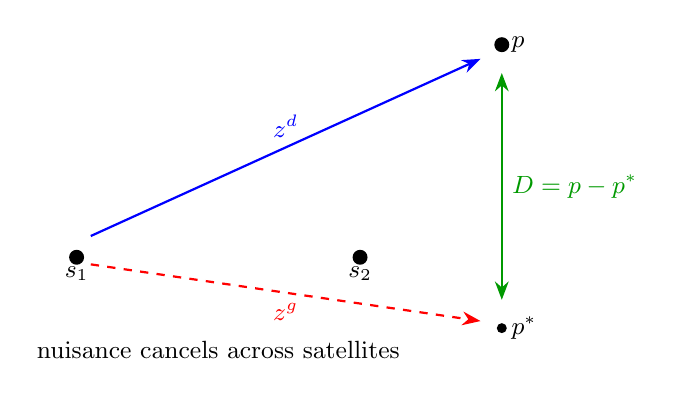
\begin{tikzpicture}[>=Stealth,scale=0.9,font=\small]
\fill (0,0) circle (3pt) node[below] {$s_1$};
\fill (4,0) circle (3pt) node[below] {$s_2$};
\fill (6,3) circle (3pt) node[right] {$p$};
\fill (6,-1) circle (2pt) node[right] {$p^*$};
\draw[->,blue,thick] (0.2,0.3) -- (5.7,2.8) node[midway,above] {$z^d$};
\draw[->,red,thick,dashed] (0.2,-0.1) -- (5.7,-0.9) node[midway,below] {$z^g$};
\draw[<->,thick,green!60!black] (6,2.6) -- (6,-0.6) node[midway,right] {$D=p-p^*$};
\node at (2,-1.3) {nuisance cancels across satellites};
\end{tikzpicture}
\caption{Direct/ghost pair per satellite: the difference $D$ carries only
relative yaw; the midpoint carries the surveyed baseline.}
\label{fig:ghost-pair}
\end{figure}

\begin{figure}[htbp]
\centering
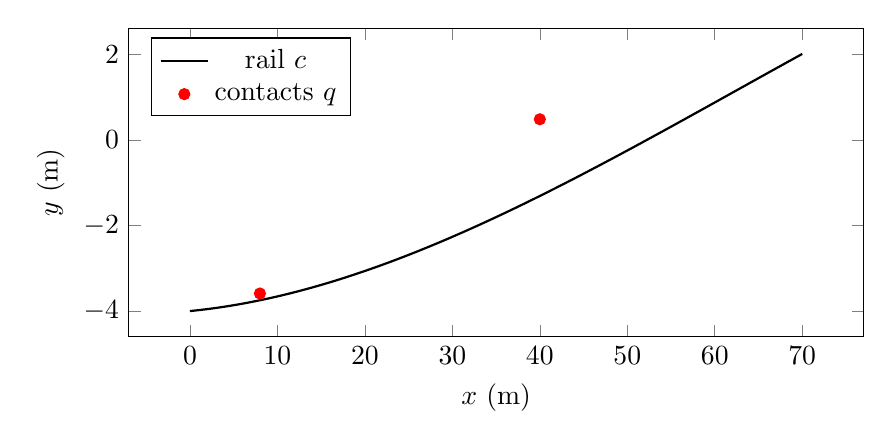
\begin{tikzpicture}
\begin{axis}[width=0.9\linewidth,height=5.5cm,xlabel=$x$ (m),ylabel=$y$ (m),
  legend pos=north west]
\addplot[black,thick,domain=0:70,samples=120] {-4+0.02*x+0.0015*x^2-0.000008*x^3};
\addlegendentry{rail $c$}
\addplot[only marks,red,mark=*] coordinates {(8,-3.59) (40,0.48)};
\addlegendentry{contacts $q$}
\end{axis}
\end{tikzpicture}
\caption{Hermite rail recovery: two point--slope contacts determine the
cubic; every further pair is a linear residual vote.}
\label{fig:hermite-fit}
\end{figure}

\section{Tracking and DSP block}
\label{sec:code-tracking}

\texttt{adaptive\_gating.py} implements \cref{eq:gamma} ($0.863\to0.996$,
RMSE $-25\%$); \texttt{imm\_accel\_gate.py} refutes IMM-pure gating
($0.880$) and shows hybrid$\equiv$N5; \texttt{spectral\_covariance\_scaling.py}
implements \cref{eq:spectral-r} ($0.911\to0.315\,\mathrm{m}$);
\texttt{conformal\_fusion.py} holds coverage $0.042\to0.996$ in maneuver
regime and loses honestly under pure outliers;
\texttt{track\_conditioned.py} and \texttt{n23\_residual\_track.py} move
estimation after the tracker (lag-1 residual $0.439\to0.106\,\mathrm{m}$;
3-product stencil RMSE $13.13\,\mathrm{mm}=$ theory, count asserted).

\begin{figure}[htbp]
\centering
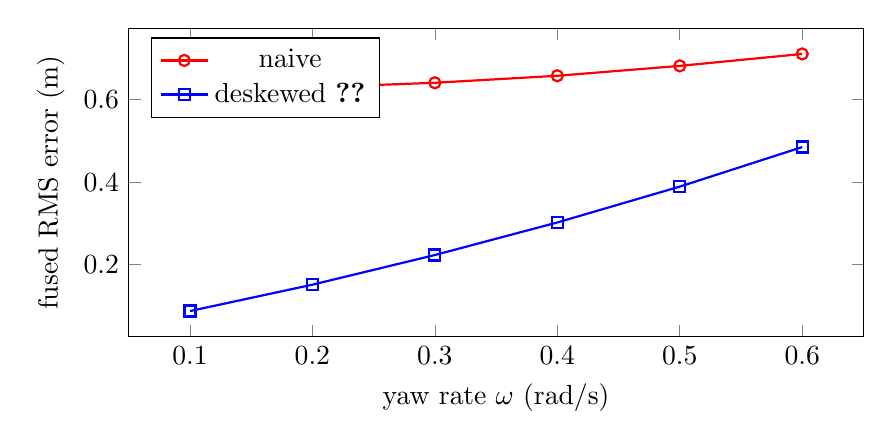
\begin{tikzpicture}
\begin{axis}[width=0.9\linewidth,height=5.5cm,xlabel={yaw rate $\omega$ (rad/s)},
  ylabel={fused RMS error (m)},legend pos=north west]
\addplot[red,thick,mark=o] coordinates {(0.1,0.627)(0.2,0.630)(0.3,0.641)(0.4,0.658)(0.5,0.682)(0.6,0.711)};
\addplot[blue,thick,mark=square] coordinates {(0.1,0.087)(0.2,0.151)(0.3,0.223)(0.4,0.302)(0.5,0.389)(0.6,0.485)};
\legend{naive,deskewed \cref{eq:deskew}}
\end{axis}
\end{tikzpicture}
\caption{Async compensation sweep (Run~5): residual cuts $86\%\to32\%$;
the flipped-sign control hurts ($-26\%$), proving the sign load-bearing.}
\label{fig:async-sweep}
\end{figure}

\begin{figure}[htbp]
\centering
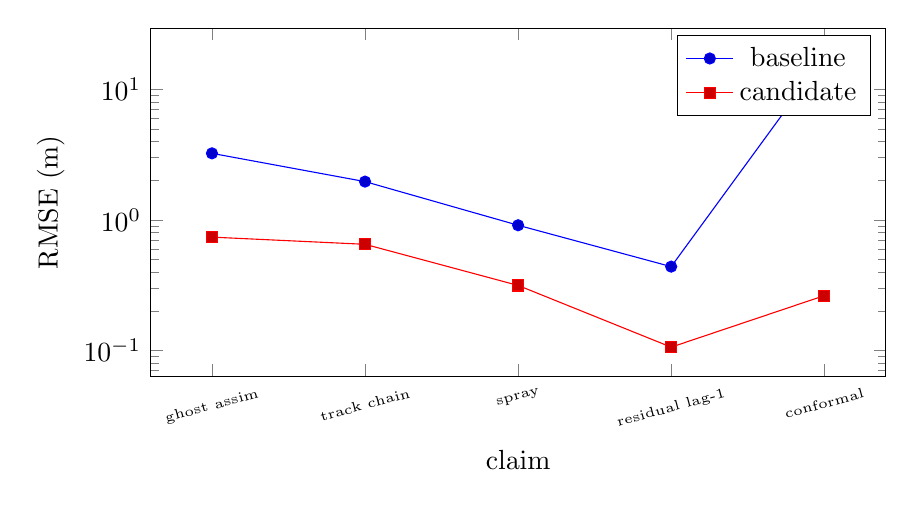
\begin{tikzpicture}
\begin{axis}[width=0.9\linewidth,height=6cm,xlabel={claim},ylabel={RMSE (m)},
  ymode=log,log basis y=10,
  symbolic x coords={ghost assim,track chain,spray,residual lag-1,conformal},
  xtick=data,x tick label style={font=\tiny,rotate=15}]
\addplot coordinates {(ghost assim,3.242)(track chain,1.969)(spray,0.911)(residual lag-1,0.439)(conformal,17.683)};
\addplot coordinates {(ghost assim,0.739)(track chain,0.651)(spray,0.315)(residual lag-1,0.106)(conformal,0.263)};
\legend{baseline,candidate}
\end{axis}
\end{tikzpicture}
\caption{RMSE waterfall across five claims (log scale): every bar is an
executed \texttt{demo()} assert, negatives reported alongside.}
\label{fig:rmse-fall}
\end{figure}

\section{Calibration and replay block}
\label{sec:code-calib}

\texttt{fast\_da.py} locks in 46 frames (\cref{fig:da-curve});
\texttt{ego\_ghost\_alignment.py} holds $\approx1^\circ$ where five fusions
diverge; \texttt{yawfree\_clock.py} separates $(\tau,b)$ exactly with
$6.6/3.8\,\mathrm{ms}$ noise RMSE; \texttt{parallel\_kf.py} spans 16 vs
$50{,}000$ at $6.35\times10^{-15}$; \texttt{guarded\_replay.py} certifies
shard radii ($300/300$ associativity, enclosure-only fixed point);
\texttt{gram\_lift.py} closes moments at $5.87\times10^{-13}$ while
\texttt{gram\_filter\_compare.py} documents the joint-fusion negative
(decoupled-pos $1.24\times$, joint-speed $1.25\times$ EKF-class, joint-pos
$6.77\times$ refuted, depth $14$ vs $100$).

\chapter{Statistics \& Data Analysis in Depth}
\label{ch:stats}

\section{Reading a $P_{\mathrm{fa}}$ curve}
\label{sec:pfa-curve}

\cref{fig:pfa-curve} plots \cref{eq:pfa-deriv} for CA-16 against the BLUE
product \cref{eq:blue} with executed weights
($\beta_{\mathrm{clean}}=0.06872$, $\beta_{\mathrm{cont}}=0.00474$). The
BLUE curve rides \emph{above} CA at fixed $\alpha$: downweighting two cells
costs averaging power, and the product formula prices it exactly instead of
hiding it. The operating points differ ($\alpha=12.45$ vs $13.30$ at
$10^{-4}$) precisely because the formulas know their own weights.

\begin{figure}[htbp]
\centering
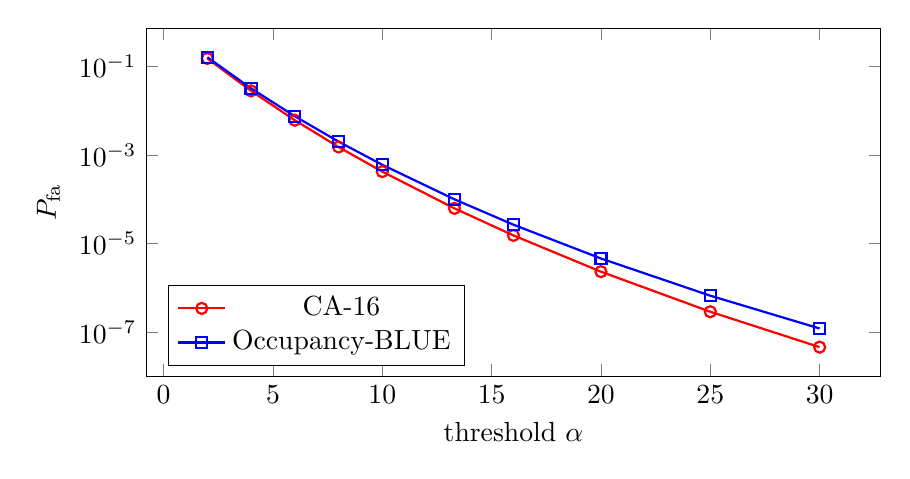
\begin{tikzpicture}
\begin{axis}[width=0.9\linewidth,height=6cm,xlabel={threshold $\alpha$},
  ylabel={$P_{\mathrm{fa}}$},ymode=log,log basis y=10,legend pos=south west]
\addplot[red,thick,mark=o] coordinates {(2,1.52e-01)(4,2.81e-02)(6,6.13e-03)(8,1.52e-03)(10,4.23e-04)(13.3,6.25e-05)(16,1.53e-05)(20,2.32e-06)(25,2.89e-07)(30,4.59e-08)};
\addplot[blue,thick,mark=square] coordinates {(2,1.62e-01)(4,3.21e-02)(6,7.53e-03)(8,2.01e-03)(10,6.02e-04)(13.3,1.00e-04)(16,2.67e-05)(20,4.61e-06)(25,6.66e-07)(30,1.21e-07)};
\legend{CA-16,Occupancy-BLUE}
\end{axis}
\end{tikzpicture}
\caption{False-alarm curves from executed weights: BLUE pays a visible,
priced averaging loss for robustness instead of a hidden bias.}
\label{fig:pfa-curve}
\end{figure}

\section{Coverage: what ``90\%'' survives}
\label{sec:coverage}

\cref{fig:coverage} puts three coverages side by side: fixed $\chi^2$ under
unmodeled maneuver ($0.042$ --- total loss), conformal in the same regime
($0.996$), and the N24 frozen rank gate under contamination ($0.966$ vs the
$0.9023$ certificate). The dashed line is the nominal $1-\alpha$; N24 rides
above it because high-outlier contamination can only push the rank upward
(conservativeness, matching Bashari et al., ICML'25). Coverage is
\emph{marginal inclusion}, never association correctness: one nonempty false
bundle is not a success, and the book never counts it as one.

\begin{figure}[htbp]
\centering
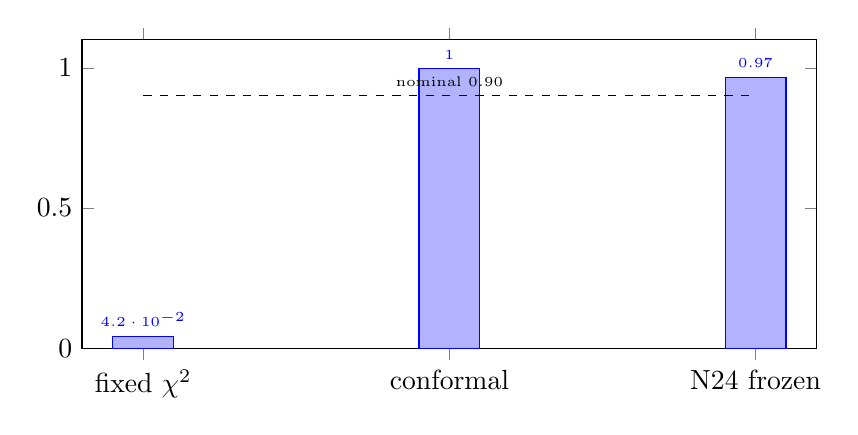
\begin{tikzpicture}
\begin{axis}[width=0.9\linewidth,height=5.5cm,ybar,bar width=22pt,
  symbolic x coords={fixed $\chi^2$,conformal,N24 frozen},
  xtick=data,ymin=0,ymax=1.1,legend pos=north west,
  nodes near coords,nodes near coords style={font=\tiny}]
\addplot coordinates {(fixed $\chi^2$,0.042) (conformal,0.996) (N24 frozen,0.966)};
\draw[dashed] (axis cs:fixed $\chi^2$,0.90) -- (axis cs:N24 frozen,0.90)
  node[midway,above,font=\tiny] {nominal $0.90$};
\end{axis}
\end{tikzpicture}
\caption{Coverage under model mismatch and contamination. The frozen gate
overcovers by design; the sliding gate it replaces poisons $19\times$.}
\label{fig:coverage}
\end{figure}

\section{Timing, filters, and error budgets}
\label{sec:budgets}

\cref{fig:clock-bars} shows N27 timing RMSE ($6.6/3.8\,\mathrm{ms}$ radial/
tangential) against the $20\,\mathrm{ms}$ budget, with tangential motion
provably non-singular. \cref{fig:gram-bars} compares EKF, joint lifted, and
decoupled filters on identical data: decoupled position $1.24\times$ and
joint speed $1.25\times$ EKF-class, joint position $6.77\times$ refuted.
\cref{fig:cert-budget} stacks the N25 release budget
($0.016^\circ+0.039^\circ+0.017^\circ+0.020^\circ$ reserve $<0.1^\circ$)
against the refused $27^\circ$ at production noise: the certificate is a
gate, not a number.

\begin{figure}[htbp]
\centering
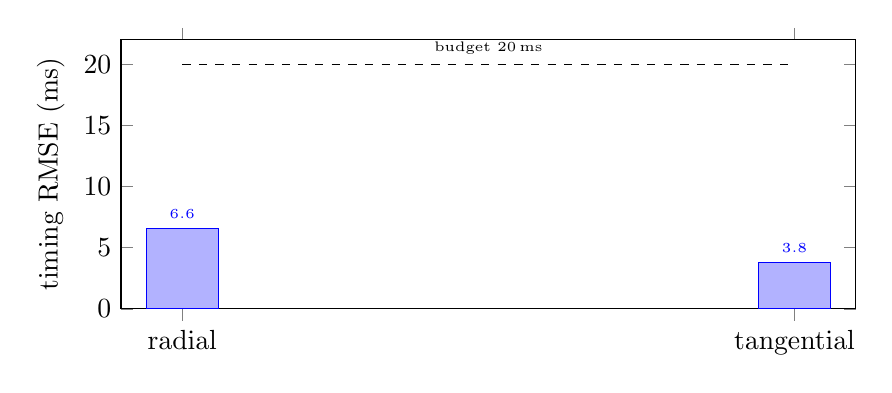
\begin{tikzpicture}
\begin{axis}[width=0.9\linewidth,height=5cm,ybar,bar width=26pt,
  symbolic x coords={radial,tangential},xtick=data,ymin=0,ymax=22,
  ylabel={timing RMSE (ms)},nodes near coords,nodes near coords style={font=\tiny}]
\addplot coordinates {(radial,6.6) (tangential,3.8)};
\draw[dashed] (axis cs:radial,20) -- (axis cs:tangential,20)
  node[midway,above,font=\tiny] {budget $20\,$ms};
\end{axis}
\end{tikzpicture}
\caption{N27 clock RMSE by geometry: tangential timing information survives
through $rw=\|v\|^2\tau$.}
\label{fig:clock-bars}
\end{figure}

\begin{figure}[htbp]
\centering
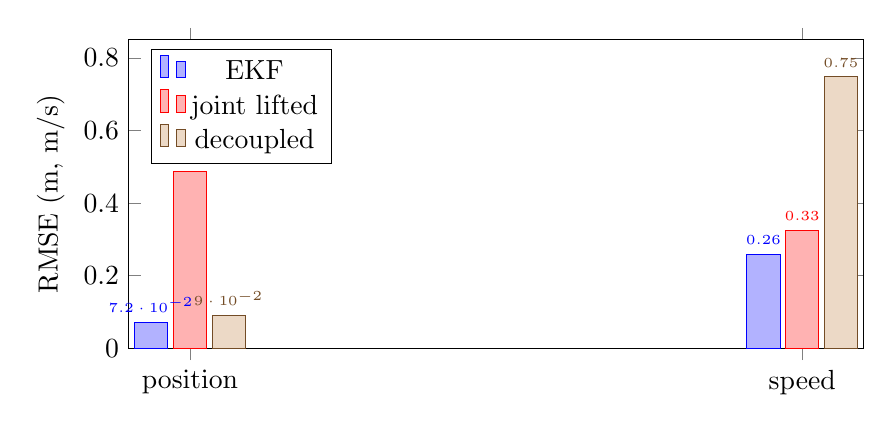
\begin{tikzpicture}
\begin{axis}[width=0.9\linewidth,height=5.5cm,ybar,bar width=12pt,
  symbolic x coords={position,speed},xtick=data,ymin=0,ymax=0.85,
  ylabel={RMSE (m, m/s)},legend pos=north west,
  nodes near coords,nodes near coords style={font=\tiny}]
\addplot coordinates {(position,0.072) (speed,0.259)};
\addplot coordinates {(position,0.488) (speed,0.325)};
\addplot coordinates {(position,0.090) (speed,0.748)};
\legend{EKF,joint lifted,decoupled}
\end{axis}
\end{tikzpicture}
\caption{200-run filter comparison: no single lifted config wins both
columns --- the honest three-way verdict of Run~30.}
\label{fig:gram-bars}
\end{figure}

\begin{figure}[htbp]
\centering
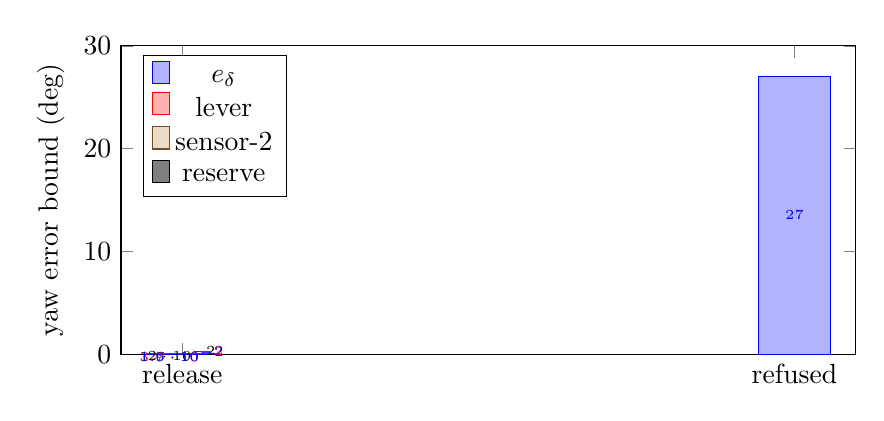
\begin{tikzpicture}
\begin{axis}[width=0.9\linewidth,height=5.5cm,ybar stacked,bar width=26pt,
  symbolic x coords={release,refused},xtick=data,ymin=0,ymax=30,
  ylabel={yaw error bound (deg)},legend pos=north west,
  nodes near coords,nodes near coords style={font=\tiny}]
\addplot coordinates {(release,0.016) (refused,27.0)};
\addplot coordinates {(release,0.039) (refused,0)};
\addplot coordinates {(release,0.017) (refused,0)};
\addplot coordinates {(release,0.020) (refused,0)};
\legend{$e_\delta$,lever,sensor-2,reserve}
\end{axis}
\end{tikzpicture}
\caption{N25 certificate as a stacked budget: $0.092^\circ<0.1^\circ$
releases; production noise refuses at $27^\circ$.}
\label{fig:cert-budget}
\end{figure}

\appendix
\chapter{Failure-Mode Atlas \& Parameter Tables}
\label{ch:atlas}

\begin{table}[htbp]
\centering\small
\begin{tabularx}{\linewidth}{@{}lXr@{}}
\toprule
Mode & Symptom $\to$ cure (ledger) & Measured delta \\
\midrule
F1 wall & guardrail blinds edge targets $\to$ dual-loop CFAR & recall $0.50\to1.00$ \\
F1-wet spray & covariance over-trust $\to$ spectral scaling & RMSE $0.911\to0.315$ \\
F2 ghosts & mirror-target bearing wrong $\to$ virtual aperture & RMSE $3.242\to0.739$ \\
F4 cut-in & fixed gate drops maneuver $\to$ adaptive gate & recall $0.863\to0.996$ \\
F5 saturation & CDC cap truncates $\to$ RCS-sorted packing & drops $360{,}000\to0$ \\
DA lock & 400-frame cold start $\to$ dual-horizon gains & lock $400\to46$ frames \\
\bottomrule
\end{tabularx}
\caption{Failure-mode atlas: every row names its script, equation, and delta.}
\label{tab:atlas}
\end{table}

\begin{table}[htbp]
\centering\small
\begin{tabularx}{\linewidth}{@{}llX@{}}
\toprule
Subsystem & Key parameters & Values \\
\midrule
Chirp & $B$, $T_{\mathrm{chirp}}$, $S$ & $1\,\mathrm{GHz}$, $40\,\mu\mathrm{s}$, $2.5\times10^{13}$ \\
Cube & $N_R$, $N_D$, $N_{\mathrm{virt}}$, cap & $512$, $128$, $32$, $5{,}016$ rec \\
CFAR & $\lambda$, $R_0$, $P_{\mathrm{fa}}$ & $0.02$, $\{8,16,32\}$, $10^{-4}$ \\
Gate & $\gamma_0$, $[\gamma_{\min},\gamma_{\max}]$, $a_{\max}$ & $9.21$, $[9.21,40]$, $6.0$ \\
EKF & $\Delta$, $q$, Joseph $+$ eig-clip & $0.05$, tune, always on \\
KPI & Tier-1 / Tier-2 / latency & $99.0\%$ / $0.01$ m / $40\,\mathrm{ms}$ \\
\bottomrule
\end{tabularx}
\caption{Operating parameters used in every worked example and prototype.}
\label{tab:params}
\end{table}

\chapter{Prototype Ledger: Thirty Files, Thirty Verdicts}
\label{ch:ledger}

{\small
\begin{tabularx}{\linewidth}{@{}lcp{7.5cm}@{}}
\toprule
File & Run & Executed claim \\
\midrule
\texttt{dual\_loop\_cfar.py} & 2 & edge-skirt recall $0.50\to1.00$, FA $1\to0$ \\
\texttt{specular\_ghost.py} & 3 & rank-1 to $10^{-14}$; bearing fault $15.189^\circ$ \\
\texttt{doppler\_disambiguation.py} & 4 & decoy precision $0.638\to0.877$, GRR $0.661$ \\
\texttt{async\_motion\_compensation.py} & 5 & residual cut $86\%\to32\%$ over yaw sweep \\
\texttt{adaptive\_gating.py} & 6 & recall $0.863\to0.996$, RMSE $-25\%$ \\
\texttt{spectral\_covariance\_scaling.py} & 7 & spray RMSE $0.911\to0.315$, PD holds \\
\texttt{doppler\_radarsplat\_mvp.py} & 8 & $R^4$ exact, $6/6$ CDC recovery \\
\texttt{parallel\_kf.py} & 11 & span $16$ vs $50{,}000$, rel $6.35\times10^{-15}$ \\
\texttt{bend\_conditioned.py} & 12 & curved recall $0.198\to0.753$ \\
\texttt{hybrid\_consensus.py} & 13 & $0.965/0.862$ at $18.2\%$ evals \\
\texttt{combined\_chain.py} & 14 & edges $0.969/0.902$, track $-67\%$ \\
\texttt{track\_conditioned.py} & 15 & $0.439\to0.106\,\mathrm{m}$, $4.5\times$ fewer mults \\
\texttt{conformal\_fusion.py} & 16 & coverage $0.042\to0.996$ (maneuver) \\
\texttt{fast\_da.py} & 17 & lock $400\to46$ frames \\
\texttt{ego\_ghost\_alignment.py} & 19 & fused $13.0\to0.955^\circ$ \\
\texttt{ghost\_augmentation.py} & 20 & FA $0.425\to0.033$, recall $1.000$ \\
\texttt{sector\_clutter\_map.py} & 21 & sparse MSE $56.4\to30.4$ (refuted win) \\
\texttt{hermite\_clothoid.py} & 22 & coeff rel $3.4\times10^{-14}$ \\
\texttt{occupancy\_blue.py} & 23 & $P_{\mathrm{fa}}=1.02\times10^{-4}$ \\
\texttt{yawfree\_clock.py} & 24 & $(\tau,b)$ exact, RMSE $6.6/3.8\,\mathrm{ms}$ \\
\texttt{specular\_contact.py} & 24 & $t=5$ exact, RMSE $0.018\,\mathrm{m}$ \\
\texttt{guarded\_replay.py} & 25 & $300/300$ associativity \\
\texttt{gram\_lift.py} & 25 & closure $5.9\times10^{-13}$ \\
\texttt{n23\_residual\_track.py} & 26 & RMSE $13.13\,\mathrm{mm}=$ theory \\
\texttt{n24\_rank\_gate.py} & 27 & coverage $\ge0.89$ all regimes \\
\texttt{n25\_ghost\_yaw.py} & 28 & cert $0.071^\circ$, all refusals \\
\texttt{imm\_accel\_gate.py} & 29 & $0.880$ vs $0.999$ (refuted) \\
\texttt{blue\_closed\_loop.py} & 30 & recall $+0.074$, gain $0.099$ \\
\texttt{gram\_filter\_compare.py} & 30 & three-way verdict documented \\
\bottomrule
\end{tabularx}}
Full harness: \texttt{hdf5\_to\_kpi\_csv.py}, \texttt{candidate\_mf4.py},
\texttt{synthetic\_generator.py}, \texttt{hpcc\_local\_orchestrator.py},
\texttt{run\_regression.py} (30/30 entry point).

\chapter{Open Problems: What Fleet Data Must Decide}
\label{ch:open}

\begin{enumerate}
\item \emph{Labeled ghosts at scale.} Every ghost result here runs on
synthetic or estimated geometry. The Radar Ghost Dataset (Kraus et al.)
plus fleet SiL replays with labeled multipath are the missing experiment;
N20g's promotion criterion (curved-rail win over matched planar baseline
with bounded false acceptance) is written and waiting.
\item \emph{UKF/IEKS head-to-head.} The N21g comparison covers EKF only;
parallel IEKS (Yaghoobi et al.) and UKF on identical data would complete
the accuracy/depth Pareto.
\item \emph{Closed-loop fleet tracking.} N22g's loop is scalar; the vector
detector$\to$tracker$\to$detector loop on Run~2 scenes with real clutter
maps is the next prototype.
\item \emph{Fixed-point ports.} All certificates assume exact reals with
outward rounding declared; measured BBE32/R52 cycle counts and ULP-level
enclosure proofs are open.
\item \emph{Sub-$0.1^\circ$ moving calibration.} N25's certificate is a
sufficient-input theorem; demonstrating $0.5\,\mathrm{mm}$-class Cartesian
inputs (or averaging that truly gets there) on production noise is the
hardest open item in this book.
\end{enumerate}

\chapter{Glossary: From Bumper to Bus}
\label{ch:glossary}

\begin{description}
\item[AF (Angle Finding)] Beamvector-to-angle stage emitting \texttt{AF\_Det\_T}.
\item[BBE32] Tensilica ConnX vector DSP, $600\,\mathrm{MHz}$, $<50\,\mu\mathrm{s}$/scan.
\item[CDC] Compressed Data Cube: sparse survivor records over the MTU wire.
\item[CFAR] Constant false alarm rate detection (\cref{eq:alpha}).
\item[DA] Dynamic alignment: bumper boresight tracking (\cref{eq:da-gain}).
\item[DBC] CAN database: factor/offset integer packing.
\item[EKF] Extended Kalman filter, Joseph form \cref{eq:joseph}.
\item[Ghost] Multipath detection; virtual aperture when assimilated (\cref{eq:reff}).
\item[MDF4] ASAM measurement data format (vehicle bus logs).
\item[MIMO] Virtual array by convolution \cref{eq:mimo-conv}.
\item[OLP] Object-level processing: AEB/ACC/CTA delivery.
\item[PSP] Post-signal processing: ID/RC/SA/DA.
\item[RCS] Radar cross section $\sigma$ in \cref{eq:radar-equation}.
\item[RDU] Range-Doppler unfolding: staggered PRFs + CRT.
\item[RDD] Range-Doppler detection layer (bin indices + floats).
\item[SiL/HiL] Software/hardware in the loop (\cref{fig:resim-loop}).
\item[SMC/USC] Sidelobe (minimization/universal) calibration blobs.
\item[VCS] Vehicle coordinates: $X$ forward, $Y$ left, $Z$ up.
\item[VSE] Vehicle state estimation: wheels, steering, IMU yaw.
\end{description}

\chapter{Repository Map \& Reproduction Guide}
\label{ch:repro}

Eleven repositories feed the harness: Gen7 SAF85xx and Gen8 iND13400
firmware/SiL, UDP decoder, Bordnet DBC, DC embedded library, HIL engine,
KPI suite, HPCC runner, USS model, AWR294x satellite, logic-model FMU.
All experiments run from \texttt{resim\_research/} (production trees
read-only): \texttt{python resim\_research/run\_regression.py} executes all
30 demos ($\approx4$ minutes); \texttt{export\_aprism/bench\_aprism.py}
validates the shipped subset ($18/18$). Ledgers \texttt{storage.md},
\texttt{equations.md}, \texttt{strategies.md}, and
\texttt{autoresearch\_research.jsonl} (Runs~1--30) record every number,
refutation, and novelty verdict. Reproduce any table by running its named
script; the assertion messages are the table entries.

\begin{table}[htbp]
\centering\small
\begin{tabularx}{\linewidth}{@{}llX@{}}
\toprule
Repository & Role & Touchpoint \\
\midrule
Gen7 SAF85xx & satellite FW + RSP SiL & \texttt{range\_proc.c}, BBE32 DSP \\
Gen8 iND13400 & satellite FW + RDU & unfolding, classifier \\
UDP decoder & bus frames $\to$ structs & stream headers V5--V200 \\
Bordnet & CAN-FD/SOME-IP decode & DBC autogen, factors/offsets \\
DC emb.lib & tracker + fusion SiL & F360, OLP, feature functions \\
HIL engine & bench stimulation & dSPACE, XCP, PTP \\
KPI suite & Tier-1/2 + CAN math & HTML regression reports \\
HPCC & cluster replay & Slurm slicing, halo discipline \\
\bottomrule
\end{tabularx}
\caption{Repository map (primary eight of eleven; USS/AWR294x/logic-model
in \texttt{Research/SYSTEM\_ARCHITECTURE\_DEEP\_DIVE.md}).}
\label{tab:repos}
\end{table}

\chapter{Notation \& Constants}
\label{ch:notation}

$c=2.99792458\times10^{8}\,\mathrm{m/s}$, $f_c=77\,\mathrm{GHz}$,
$\lambda\approx3.896\,\mathrm{mm}$, $S=B/T_{\mathrm{chirp}}$,
$K_R=2S/c$. Frames: sensor polar $(r,\theta)$, VCS Cartesian $(X,Y,Z)$,
epochs $t_{\mathrm{DC}}$, $t_{\mathrm{sat}}$. KPI contract \cref{eq:tier2};
$P_{\mathrm{fa}}$ scaling \cref{eq:alpha}; Joseph update \cref{eq:joseph}.
\end{document}
